% ==============================================================================
% CAPÍTULO 3: MODELAGEM MATEMÁTICA DO SUBSISTEMA ELÉTRICO E DE ARMAZENAMENTO
% ==============================================================================
\section{MODELAGEM MATEMÁTICA DO SUBSISTEMA ELÉTRICO E DE ARMAZENAMENTO}

A operação contínua e segura de centros de dados orbitais voltados ao processamento massivo de inteligência artificial requer uma infraestrutura de potência de alta densidade, capaz de conciliar potências na faixa de dezenas de quilowatts por satélite com as severas restrições de massa, volume e dissipação térmica intrínsecas ao voo espacial. Este capítulo descreve a modelagem teórico-computacional do Subsistema de Suprimento de Energia Elétrica (\textit{Electrical Power System} -- EPS), da distribuição em alta tensão à dinâmica do BESS. As rotinas encontram-se descritas no Apêndice~C. Os gráficos e resultados quantitativos existentes nesta versão ainda não foram regenerados após a revisão das capacidades e cenários; devem ser tratados como resultados legados até nova execução reproduzível.

\subsection{Arquitetura do Barramento de Potência e Balanço Geral de Cargas}
\label{sec:arquitetura_barramento_balanco}

A concepção elétrica da plataforma adota uma topologia de barramento de alta tensão em corrente contínua (\textit{High-Voltage Direct Current} -- HVDC) com nível nominal primário padronizado em $V_{nom} = 400\text{ VDC}$ [CALCULADO], rigorosamente balizado pelas diretrizes de mitigação de descargas por efeito corona e arcos sustentados por plasma estabelecidas na norma NASA-HDBK-4007A (NASA, 2026; Anexo~B). A seleção dessa magnitude de tensão decorre do compromisso termodinâmico e estrutural de minimizar as perdas ôhmicas de condução nos cabos de distribuição que interligam as asas solares desdobráveis ao corpo central do rack, evitando o aumento proibitivo de massa de condutores que ocorreria em barramentos espaciais convencionais de 28~VDC ou 100~VDC. Esta classe de tensão reduz a corrente nominal de alimentação do nó de IA de 20~kW para aproximadamente 50~A a 55~A, viabilizando uma redução de mais de 92\% nas perdas ôhmicas de distribuição por efeito Joule.

O balanço instantâneo de potência no barramento primário é expresso pela igualdade funcional:
\begin{equation}
    P_{pv}(t) + P_{bat}(t) = P_{IT}(t) + P_{OISL}(t) + P_{aux}(t) + P_{loss,conv}(t)
    \label{eq:balanco_potencia_global}
\end{equation}
onde $P_{pv}(t)$ é a potência líquida entregue pelo gerador fotovoltaico após o rastreamento de máxima potência, $P_{bat}(t)$ representa a potência de carga ($P_{bat} < 0$) ou descarga ($P_{bat} > 0$) do banco de baterias, $P_{IT}(t)$ sintetiza a demanda computacional agregada dos nós de processamento neural ($2\text{ a }20\text{ kW}$ por rack), $P_{OISL}(t)$ expressa o consumo dos módulos de comunicação laser inter-satélite, $P_{aux}(t)$ consolida as cargas de instrumentação, aviônica e bombas de arrefecimento ($560\text{ W}$ contínuos), e $P_{loss,conv}(t)$ agrega a totalidade das perdas estáticas e dinâmicas nos estágios de conversão eletrônica.

Para uma infraestrutura modular em cluster orbital, a comunicação e sincronização de tensores neurais entre nós cooperantes é viabilizada por quatro terminais ópticos inter-satélite (\textit{Optical Inter-Satellite Links} -- OISL) operando no comprimento de onda de $\lambda = 1550\text{ nm}$ [PROVISÓRIO]. Cada terminal consome continuamente $110\text{ W}$ de potência elétrica para alimentação de diodos laser de bombeamento, amplificadores ópticos EDFA e atuadores de espelhos rápidos de direcionamento (\textit{Fast Steering Mirrors} -- FSM). Considerando a eficiência de conversão eletro-óptica de $\eta_{eo} = 22\%$ [DEPENDENTE DE HARDWARE], a fração restante de $78\%$ da potência consumida ($85{,}8\text{ W}$ por terminal, totalizando $Q_{OISL} = 343{,}2\text{ W}$) é integralmente convertida em calor interno residual no interior do chassi, devendo ser incorporada ao balanço térmico que onera o sistema de rejeição radiativa da carcaça.

\subsubsection{Otimização Eletromecânica da Cablagem e Balanço Orbital do BESS}

A definição do material condutor obedece ao compromisso de redução de massa de lançamento. Comparando condutores de Cobre Eletrolítico ($Cu$, densidade $\delta_{Cu} = 8{,}96\text{ g/cm}^3$, $\rho_{Cu} = 1{,}72 \times 10^{-8}\ \Omega\cdot\text{m}$) com ligas de Alumínio Aeronáutico ($Al$ 6061-T6, densidade $\delta_{Al} = 2{,}70\text{ g/cm}^3$, $\rho_{Al} = 2{,}82 \times 10^{-8}\ \Omega\cdot\text{m}$), a relação analítica de massa para uma mesma resistência elétrica total (cuja dedução passo a passo é apresentada no Apêndice~B.1) comprova que o condutor de alumínio proporciona uma redução líquida de 50{,}6\% na massa total de cablagem frente ao cobre ($M_{Al}/M_{Cu} \approx 0{,}494$), justificando a sua adoção conforme as normas NASA-SP-8005 (NASA, 1972), ECSS-Q-ST-70-26C (ECSS, 2020) e MIL-W-5088L. Adotou-se o cabo AWG 4 ($21{,}15\text{ mm}^2$, capacidade nominal de 80~A no vácuo) com comprimento de chicote interno de $L_{cabo} = 4{,}5\text{ m}$ ($R_{dist,nom} = 14\text{ m}\Omega$, variando no pior caso degradado EOL a $90^\circ\text{C}$ até $R_{dist} = 50\text{ m}\Omega$). A indutância parasita distribuída (NASA-HDBK-4007A) é de $L_{dist,nom} = 1{,}8\ \mu\text{H}$, atingindo no pior caso de laço de chicote $L_{dist} = 4{,}0\ \mu\text{H}$.

O banco de baterias (\textit{Battery Energy Storage System} -- BESS) possui topologia de 108 células Li-ion NMC em série ($108\text{S}1\text{P}$ de $22{,}5\text{ Ah}$), capacidade nominal unitária de $E_{bat,no} = 9{,}0\text{ kWh}$ ($399{,}6\text{ V}$ nominais, massa de $60\text{ kg}$) e faixa operacional entre $V_{UV} = 324\text{ V}$ ($3{,}0\text{ V/célula}$, corte crítico por subtensão) e $V_{OV} = 442{,}8\text{ V}$ ($4{,}1\text{ V/célula}$, teto de sobretensão) (NASA, 2021). A resistência interna do banco $R_0$, balizada por ensaios de qualificação espacial (JUN et al., 2020), foi parametrizada em três níveis: $32\text{ m}\Omega$ (BOL quente a $30^\circ\text{C}$), $45\text{ m}\Omega$ (nominal a $20^\circ\text{C}$) e $85\text{ m}\Omega$ (EOL frio a $5^\circ\text{C}$). A dinâmica do Estado de Carga ($SoC$) e a tensão terminal instantânea $V_{bus}(t)$ são regidas por:
\begin{align}
    \frac{dSoC(t)}{dt} &= \begin{cases} -\dfrac{P_{bat}(t)}{\eta_{dis} E_{bat,nom}}, & P_{bat}(t) \ge 0 \quad \text{(descarga)} \\[0.2cm] -\dfrac{\eta_{ch} P_{bat}(t)}{E_{bat,nom}}, & P_{bat}(t) < 0 \quad \text{(carga)} \end{cases} \label{eq:bess_dinamica} \\
    V_{bus}(t) &= V_{oc}(SoC,T_{bat}) - I_{bat}(t)\left[R_0+R_{dist}\right] - V_{p1}(t)-V_{p2}(t) \label{eq:vbus_bess_dinamica}
\end{align}
Adota-se $P_{bat}>0$ na descarga e $P_{bat}<0$ na carga, com $I_{bat}>0$ na descarga. Na integração contínua, $E_{bat,nom}$ deve estar em joules, $P_{bat}$ em watts e $t$ em segundos; $\eta_{ch}$ e $\eta_{dis}$ permanecem parâmetros até serem sustentados por fonte ou dados de célula. A expressão de $V_{bus}$ inclui a resistência interna do pack, a resistência de distribuição e os estados de polarização do modelo DP.

\subsubsection{Dinâmica Transitória sob Degraus de IA e Estabilidade CPL}

Os aceleradores neurais locais comportam-se perante o barramento de 400~V como Cargas de Potência Constante (\textit{Constant Power Loads} -- CPL), exibindo impedância incremental negativa $Z_{in,CPL} = -V_{bus}^2 / P_{load}$ que tende a desestabilizar o circuito de distribuição caso o critério de Middlebrook (MIDDLEBROOK, 1976) seja violado ($\|Z_{out,source}\| \ll \|Z_{in,load}\|, \forall \omega$). A dinâmica acoplada RLC no domínio do tempo é expressa por:
\begin{equation}
    \frac{dI_{bus}(t)}{dt} = \frac{V_{src} - V_{bus}(t) - R_{dist} I_{bus}(t)}{L_{dist}}, \qquad \frac{dV_{bus}(t)}{dt} = \frac{I_{bus}(t) - \frac{P_{load}(t)}{V_{bus}(t)}}{C_{bus}}
    \label{eq:rlc_estado}
\end{equation}
cujo fator de amortecimento intrínseco é $\zeta = \frac{R_{dist}}{2}\sqrt{\frac{C_{bus}}{L_{dist}}}$ e a frequência natural é $f_0 = \frac{1}{2\pi \sqrt{L_{dist} C_{bus}}}$.

A Figura~\ref{fig:dinamica_barramento_bess} consolida o balanço energético multianel do BESS de 9,0~kWh ao longo de 5 órbitas consecutivas nos cenários de 500~km (LEO com eclipse máximo de 35,8~min), 700~km (SSO com eclipse sazonal de 18,8~min) e 35.786~km (GEO com eclipse de equinócio de 72,0~min).

\begin{figure}[htbp]
    \centering
    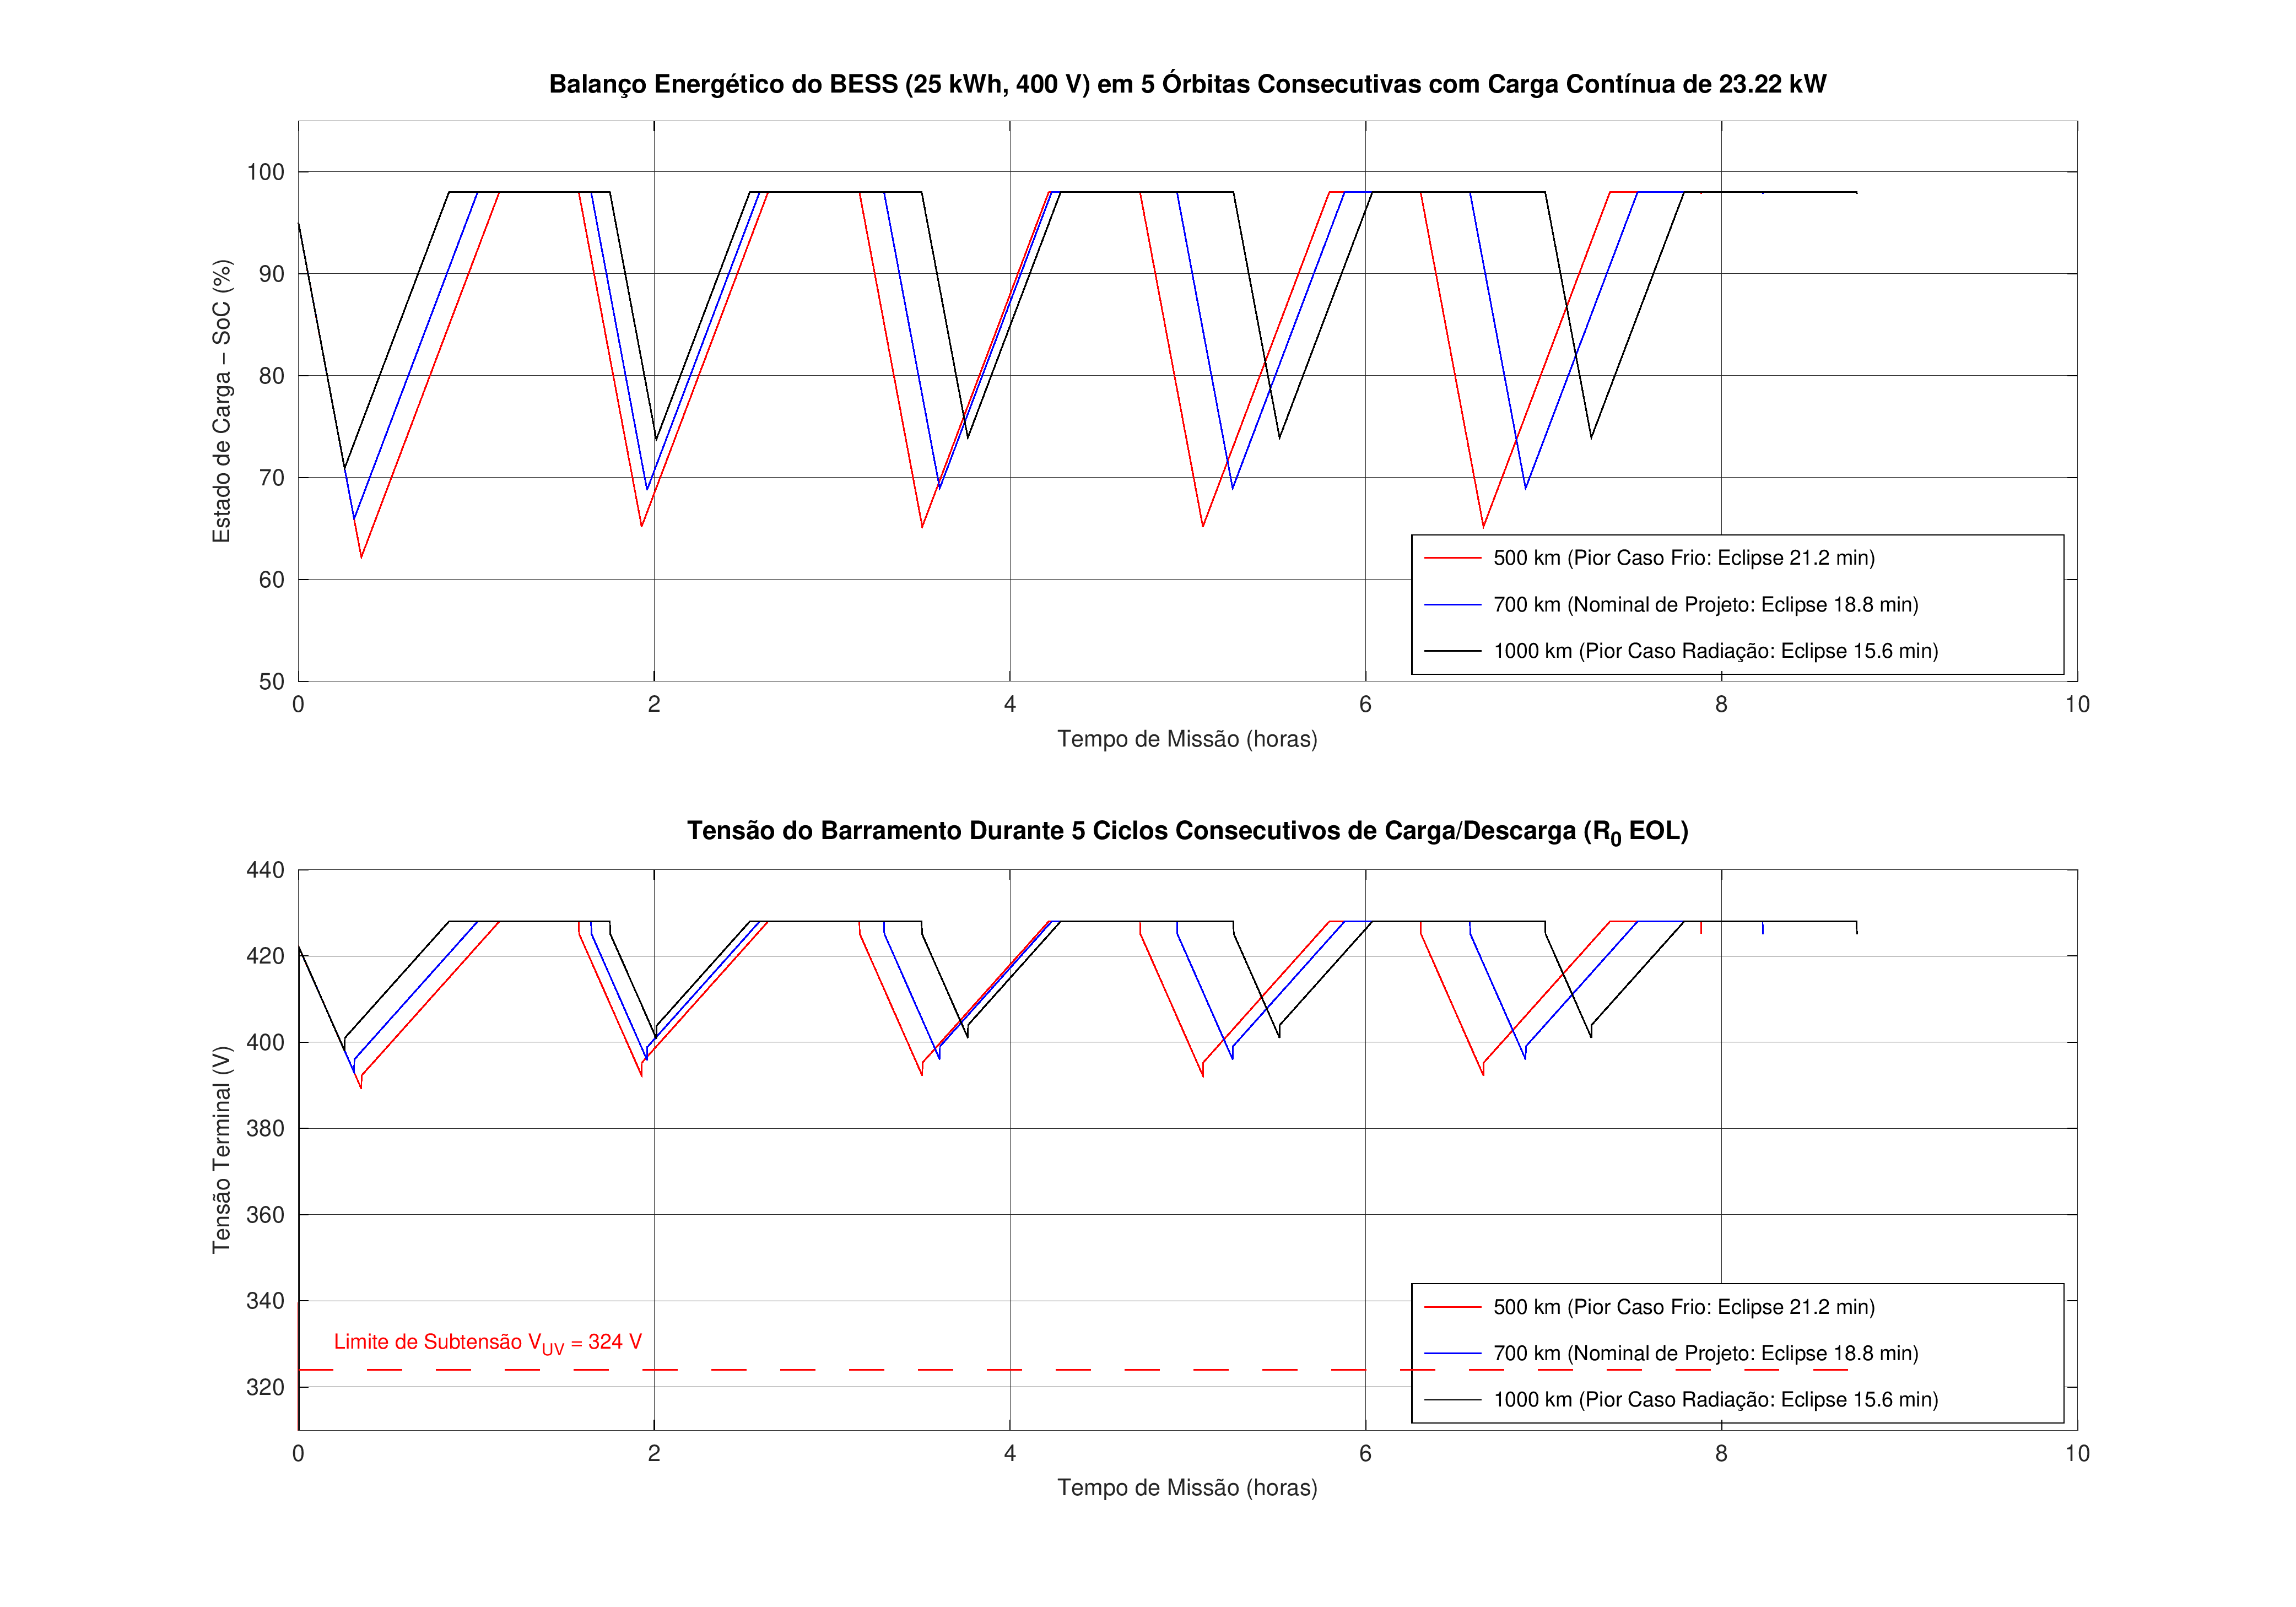
\includegraphics[width=0.82\textwidth]{figuras/figura_3_1_balanco_orbital_bess.png}
    \caption{Balanço energético e dinâmica de tensão do BESS (9,0~kWh, 400~V) ao longo de 5 órbitas consecutivas com gestão de carga: evolução do Estado de Carga ($SoC \ge 20\%$) e perfil de tensão terminal nos cenários LEO (500~km), SSO (700~km) e GEO (35.786~km).}
    \label{fig:dinamica_barramento_bess}
\end{figure}

A análise do balanço energético em eclipse exige a distinção conceitual rigorosa entre a operação nominal sob controle ativo e o modo de contingência por falha de gestão:
\begin{enumerate}[label=(\alph*),leftmargin=*]
    \item \textbf{Modo de Falha BAT-F01 (Falha do TEMS / Sobrecarga sem Modulação):} Caso o sistema de gerenciamento térmico-energético (TEMS) falhe em modular a carga de processamento e mantenha o nó operando em plena potência de $20\text{ kW}$ durante os $35{,}8\text{ min}$ de eclipse de LEO, a energia requerida totaliza $(20\text{ kW} + 0{,}56\text{ kW}) \times (35{,}8/60)\text{ h} \approx 12{,}27\text{ kWh}$, superando em $+36{,}3\%$ a capacidade instalada de $9{,}0\text{ kWh}$ ($32{,}4\text{ MJ}$). A simulação dinâmica demonstra que, sem a saturação artificial numérica outrora empregada, o banco de baterias sofre exaustão completa e atinge o corte crítico de subtensão ($V_{UV} = 324{,}0\text{ V}$, com colapso terminal em $318{,}5\text{ V}$) aos exatos $19{,}9\text{ minutos}$ de eclipse, provocando o desligamento forçado por proteção primária do BMS (\textit{Modo de Falha BAT-F01}). Isso comprova a necessidade mandatória da gestão ativa de carga;
    \item \textbf{Regime Nominal com Modulação de Carga (Controle TEMS):} No regime nominal de projeto, o TEMS restringe o processamento durante o período de sombra aos tetos de \textit{throttling} compatíveis com a reserva de $9{,}0\text{ kWh}$: em LEO (500~km), a carga computacional é modulada para $6{,}5\text{ kW}$ nominais ($+560\text{ W}$ de aviônica/cargas essenciais $= 7{,}06\text{ kW}$ total), consumindo apenas $4{,}21\text{ kWh}$ ($DoD = 49{,}54\%$), mantendo o Estado de Carga mínimo em confortáveis $SoC = 50{,}46\%$ e a tensão terminal em $382{,}4\text{ V}$; em SSO (700~km, $18{,}8\text{ min}$ de eclipse), a carga é mantida em $18{,}0\text{ kW}$ ($+560\text{ W} = 18{,}56\text{ kW}$), consumindo $5{,}82\text{ kWh}$ ($SoC_{min} = 31{,}56\%$, $V_{min} = 357{,}2\text{ V}$); e em GEO (35.786~km, $72{,}0\text{ min}$ de eclipse), modula-se para $4{,}5\text{ kW}$ ($+560\text{ W} = 5{,}06\text{ kW}$), consumindo $6{,}07\text{ kWh}$ ($SoC_{min} = 28{,}63\%$, $V_{min} = 356{,}8\text{ V}$). Em todos os cenários nominais, o piso normativo de $SoC \ge 20\%$ é rigorosamente atendido com ampla margem operacional;
    \item \textbf{Recarga Solar e Proteção por Controle CC-CV:} Durante a insolação solar, o conversor Buck do gerador fotovoltaico restabelece o SoC para 100\% sob controle estrito em dois estágios: na fase inicial de Corrente Constante (CC), a recarga é limitada a $1{,}0\text{C}$ ($22{,}5\text{ A}$ por nó); ao atingir $V_{OV} = 442{,}8\text{ V}$ ($4{,}10\text{ V/célula}$), a malha transiciona autonomamente para Tensão Constante (CV), mantendo $V_{bus} \le 442{,}8\text{ V}$ e eliminando o risco de sobretensão eletroquímica (\textit{Falha BAT-F02}).
\end{enumerate}

\subsubsection{Falhas Catastróficas: Curto-Circuito Franco, Religamentos e Acoplamento Térmico}

Para analisar contingências destrutivas, modelou-se o curto-circuito franco ($R_{sc} = 1\text{ m}\Omega$, $C_{bus} = 1{,}5\text{ mF}$, $L_{dist} = 4{,}0\ \mu\text{H}$) com atuação do interruptor SSPC em SiC MOSFET ($I^2t_{lim} = 1500\text{ A}^2\text{s}$; ECSS, 2008) e acoplamento térmico ao chassi:
\begin{equation}
    I^2t = \int_0^{t_{clear}} I_{sc}^2(t) \, dt, \qquad C_{th,elec} \frac{dT_{elec}(t)}{dt} = P_{loss,conv}(t) + Q_{OISL} - G_{th} \left[ T_{elec}(t) - T_{rad} \right]
    \label{eq:curto_termico_acoplado}
\end{equation}
onde $C_{th,elec} = 18000\text{ J/K}$ ($\approx 20\text{ kg}$ de alumínio), $Q_{OISL} = 343{,}2\text{ W}$ e $G_{th} \in [80, 120, 160]\text{ W/K}$.

A Figura~\ref{fig:falhas_eletrotermicas_sspc} consolida a resposta de falta e o acoplamento térmico contínuo.

\begin{figure}[htbp]
    \centering
    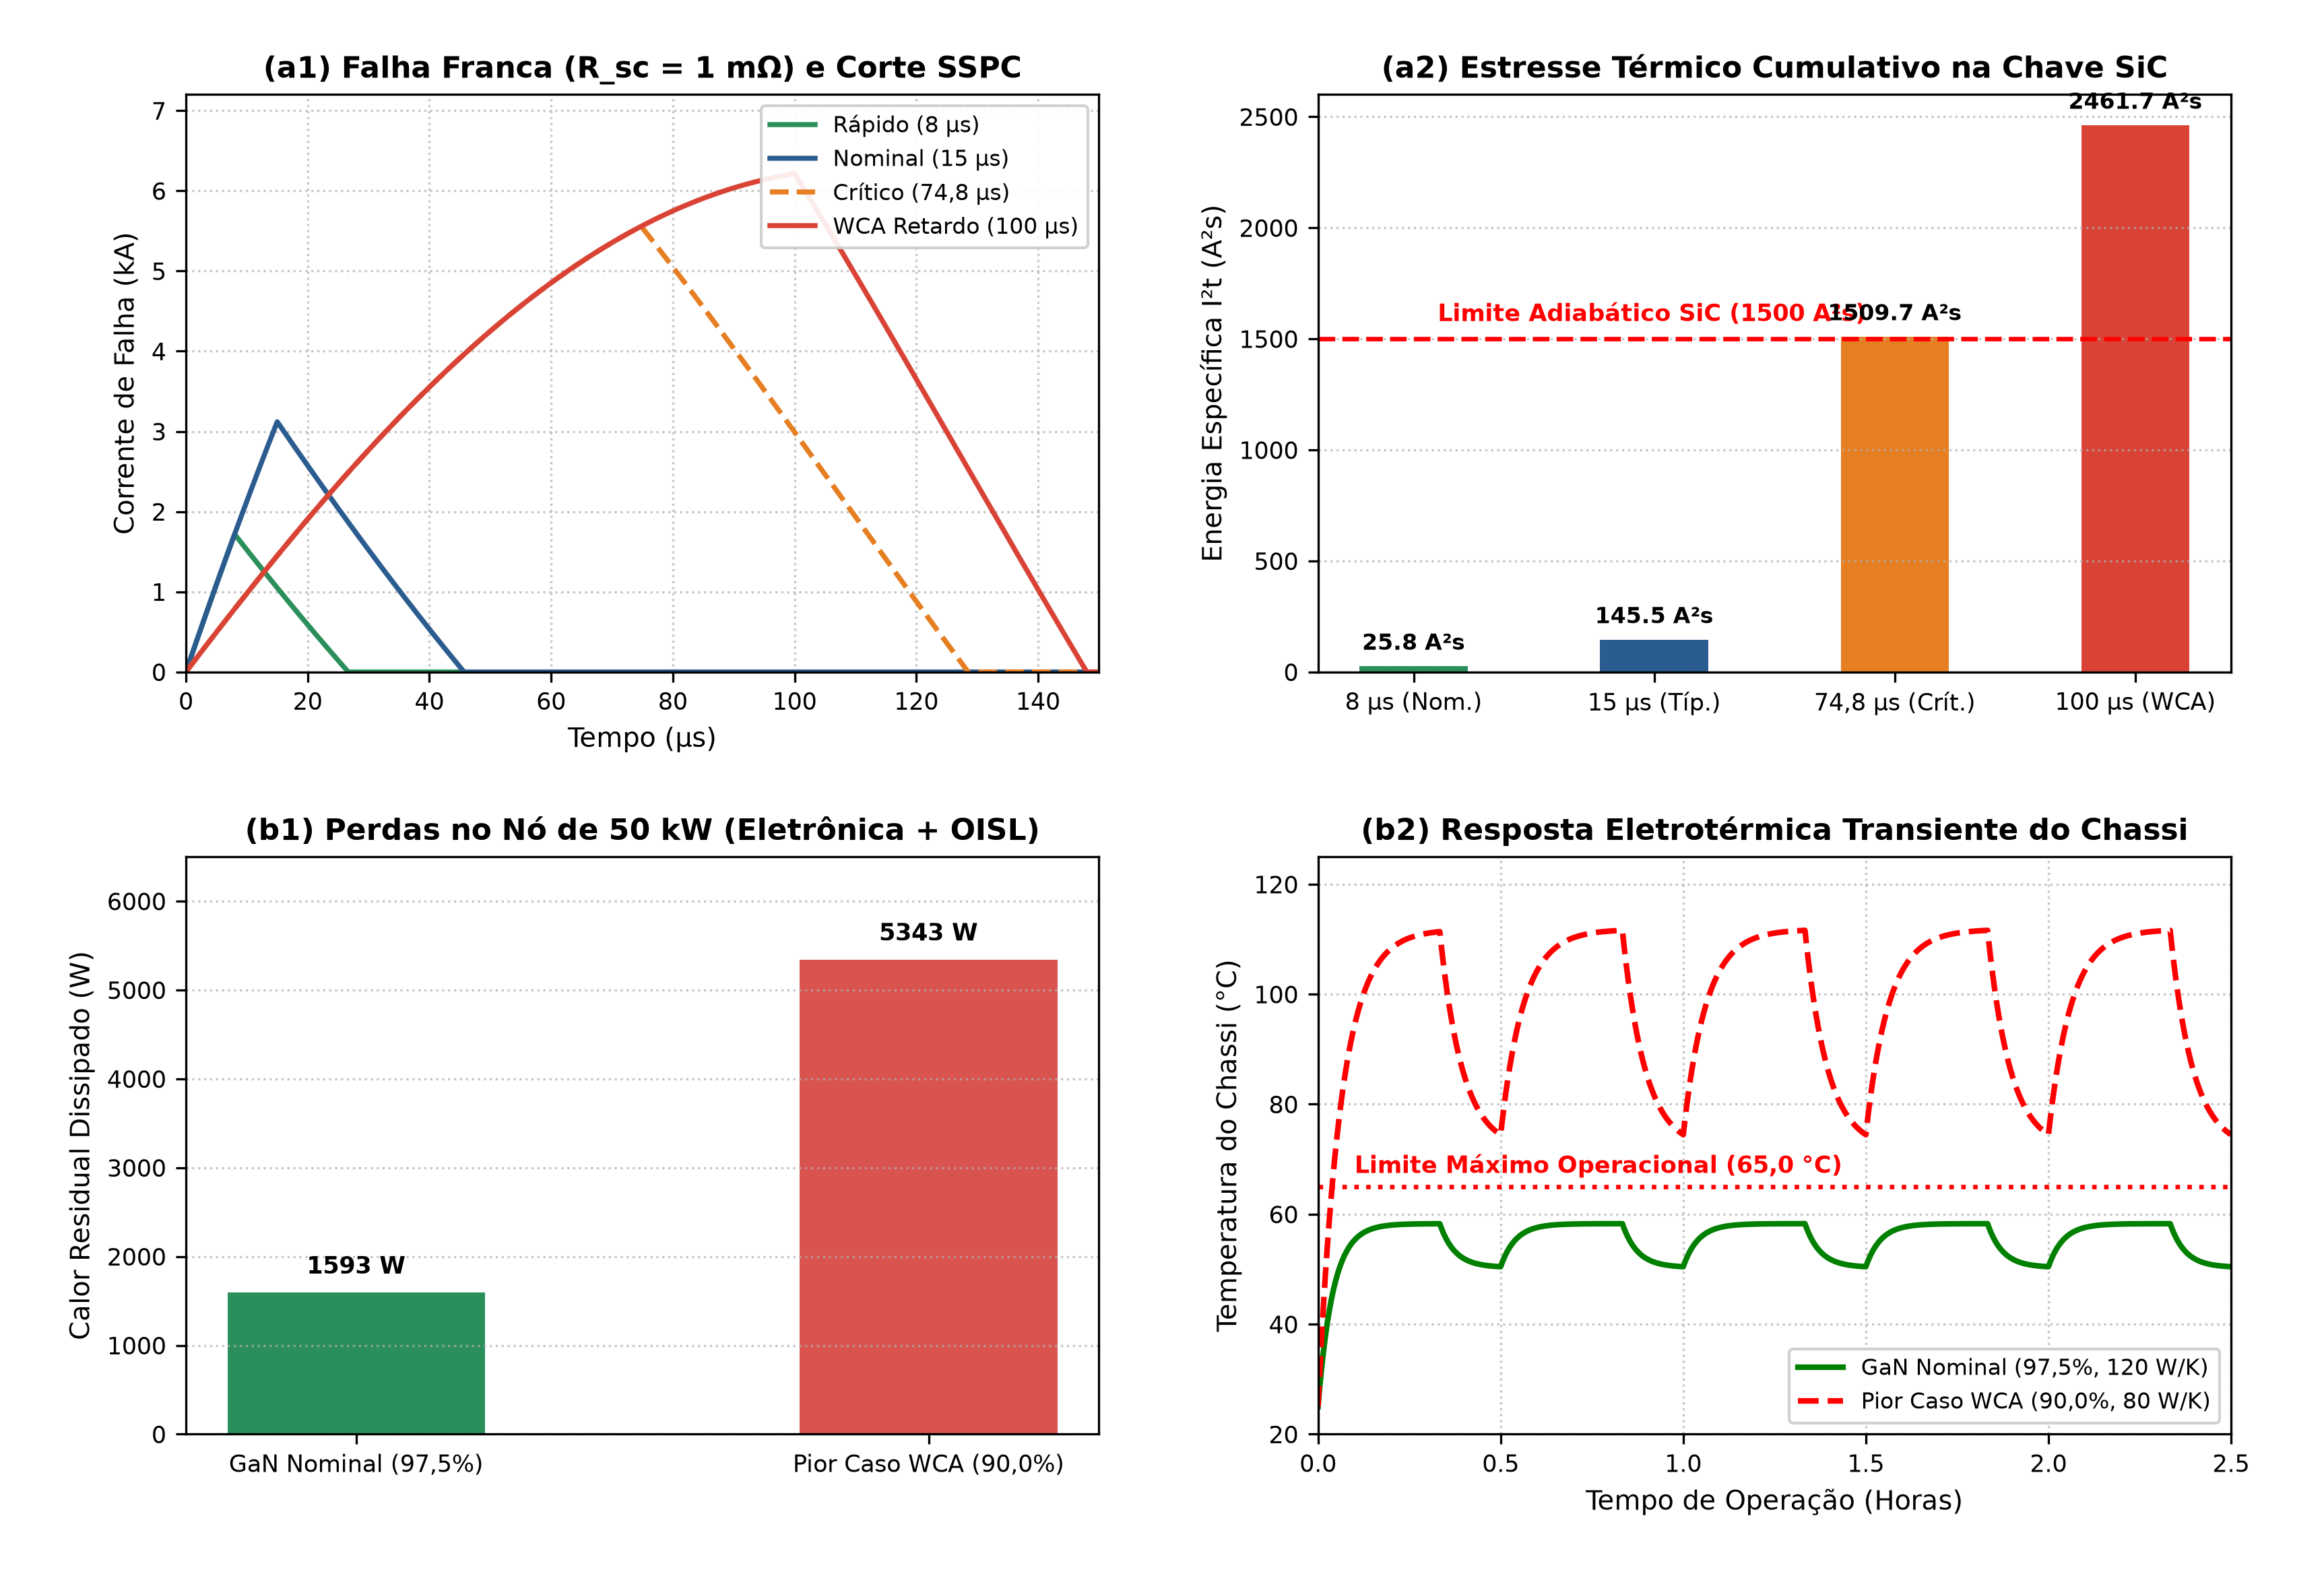
\includegraphics[width=0.82\textwidth]{figuras/figura_3_2_falhas_eletrotermicas_sspc.png}
    \caption{Análise de falhas catastróficas e acoplamento térmico do barramento HVDC de 400~V: (a1) corrente de curto-circuito franco ($R_{sc} = 1\text{ m}\Omega$) para tempos de corte de $8\ \mu\text{s}$, $15\ \mu\text{s}$ e $100\ \mu\text{s}$; (a2) estresse cumulativo ($I^2t$) confrontado com o limite adiabático do SiC ($1500\text{ A}^2\text{s}$); (b1) perdas térmicas no nó de 50~kW comparando GaN nominal a $97{,}5\%$ ($1593\text{ W}$) versus pior caso a $90{,}0\%$ ($5343\text{ W}$); (b2) resposta eletrotérmica do chassi ao longo de 2,5~h ($58{,}27^\circ\text{C}$ estável vs. $111{,}61^\circ\text{C}$ em runaway).}
    \label{fig:falhas_eletrotermicas_sspc}
\end{figure}

A análise numérica do curto-circuito revela duas conclusões técnicas críticas para o projeto de proteção do barramento primário de 400~V:
\begin{itemize}[leftmargin=*]
    \item \textbf{Conclusão Técnica 1 (Limite Adiabático de Fusão do SiC MOSFET):} A varredura temporal paramétrica demonstra que o limite adiabático do interruptor de estado sólido ($I^2t_{lim} = 1500\text{ A}^2\text{s}$, conforme ECSS-E-ST-20-20C e MIL-HDBK-338B) é atingido sob condições de pior caso (WCA: $L_{dist} = 4{,}0\ \mu\text{H}$, $C_{bus} = 1{,}5\text{ mF}$, $R = 15\text{ m}\Omega$) para um tempo de retardo de abertura crítico de exatamente $t_{trip,crit} = 74{,}8\ \mu\text{s}$ (atingindo corrente de pico de $5{,}55\text{ kA}$ e integral Joule de $1506{,}2\text{ A}^2\text{s}$). Sob um retardo severo de $t_{trip} = 100\ \mu\text{s}$, a corrente atinge pico de $6{,}21\text{ kA}$ e energia cumulativa de $I^2t = 2461{,}7\text{ A}^2\text{s}$ ($+64{,}1\%$ acima do limite de fusão), provocando a destruição térmica irreversível do semicondutor e exigindo bloqueio definitivo (\textit{lockout}) para impedir reignição catastrófica. Em contrapartida, o tempo de corte nominal do detector analógico de sobrecorrente ($t_{trip} \in [8, 15]\ \mu\text{s}$) restringe a energia a $I^2t \le 145{,}5\text{ A}^2\text{s}$, proporcionando margem de segurança superior a dez vezes frente à ruptura térmica. Ademais, quando o ramo da bateria ($R_0 \approx 45\text{ m}\Omega$, $L_{bat} \approx 2{,}5\ \mu\text{H}$) atua em paralelo com o capacitor de barramento durante o curto franco, a tensão de barramento é sustentada e eleva a corrente de falta para $I_{peak} = 6{,}41\text{ kA}$ e $I^2t = 2636{,}2\text{ A}^2\text{s}$, reforçando a gravidade do evento caso o trip rápido não atue.
    \item \textbf{Conclusão Técnica 2 (Limite de Sobretensão Indutiva e Ruptura Dielétrica):} Em caso de falha ou ausência do circuito de grampeamento por snubber/TVS com desligamento não-controlado do gate-driver ($\tau_{ext} = 0{,}5\ \mu\text{s}$), a tensão de ruptura do SiC MOSFET ($V_{ds,max} = 1200\text{ V}$) é superada com retardo de apenas $t_{trip} = 1{,}00\ \mu\text{s}$ ($1000\text{ ns}$), bastando uma corrente de corte de apenas $100\text{ A}$ a $200\text{ A}$ para induzir sobretensão superior a $1200\text{ V}$ ($V_{spike} = V_{bus} + L_{dist} \frac{di}{dt} = 400 + 4{,}0\times 10^{-6} \times \frac{100}{0{,}5\times 10^{-6}} = 1200\text{ V}$). Para o caso WCA de $100\ \mu\text{s}$ ($I_{peak} = 6{,}21\text{ kA}$), a sobretensão teórica não-grampeada alcançaria destrutivos $50{,}1\text{ kV}$ ($11{,}99\text{ kV}$ sob corte moderado), perfurando instantaneamente a camada epitaxial de óxido de silício. Torna-se, portanto, requisito obrigatório de projeto o emprego de diodos TVS de resposta sub-nanossegundo com nível de grampeamento fixado em $550\text{ V}$ e/ou circuito de gate com desligamento suave progressivo (\textit{soft turn-off}) garantindo $\tau_{ext} \ge 31{,}1\ \mu\text{s}$.
\end{itemize}

Em regime térmico contínuo, a eletrônica GaN nominal dissipa $1593\text{ W}$ estabilizando o chassi em seguros $58{,}27^\circ\text{C}$ sob $G_{th} = 120\text{ W/K}$, enquanto a falha degradada a $90\%$ dissipa $5343\text{ W}$ sob $80\text{ W/K}$, escalando a estrutura para $111{,}61^\circ\text{C}$ e violando o teto operacional de $65{,}0^\circ\text{C}$ (\textit{Falha ET-F01}).

O Quadro~\ref{quadro:parametros_barramento_sintese} resume os parâmetros essenciais de projeto e estresse WCA do barramento HVDC, remetendo ao Apêndice~A para o catálogo cadastral exaustivo de propriedades.

\begin{table}[!ht]
\centering
\small
\renewcommand{\arraystretch}{0.85}
\caption{Parâmetros essenciais de projeto e análise de estresse extremo (WCA) do barramento HVDC de 400~V.}
\label{quadro:parametros_barramento_sintese}
\resizebox{0.95\textwidth}{!}{%
\begin{tabular}{lccccp{5.5cm}}
\hline
\textbf{Parâmetro de Decisão} & \textbf{Símbolo} & \textbf{Mínimo} & \textbf{Nominal} & \textbf{Máximo} & \textbf{Referência / Justificativa Normativa} \\ \hline
Tensão do Barramento HVDC & $V_{bus}$ & 324,0~V & 400,0~V & 442,8~V & NASA-HDBK-4007A (NASA, 2026); Anexo~B \\
Potência Total Demandada & $P_{load}$ & 2,9~kW & 21,5~kW & 23,2~kW & IA (2-20 kW), OISL (440 W), aviónica (560 W) \\
Eficiência Global de Conversão & $\eta_{conv}$ & 90,0\% & 97,5\% & 98,2\% & 90,0\% conservador térmico; GaN/SiC nominal \\
Capacidade e Resistência do BESS & $E_{bat}, R_0$ & 8,4~kWh / 32~m$\Omega$ & 9,0~kWh / 45~m$\Omega$ & 9,6~kWh / 85~m$\Omega$ & Pack 108S1P; energia coerente com 21/22,5/24~Ah a 399,6~V \\
Resistência de Distribuição & $R_{dist}$ & 10~m$\Omega$ & 14~m$\Omega$ & 50~m$\Omega$ & Cabos de alumínio AWG 4 (redução 50,6\% massa) \\
Fator de Amortecimento & $\zeta$ & 0,097 & 0,358 & 0,484 & $\zeta = 0{,}097$ sob $R_{dist} = 10\text{ m}\Omega$ (subamortecido) \\
Indutância e Capacitância & $L_{dist}, C_{bus}$ & 1,0~$\mu$H / 1,5~mF & 1,8~$\mu$H / 4,7~mF & 4,0~$\mu$H / 6,0~mF & EOL degradado e pior arranjo de chicotes \\
Tempo de Corte do SSPC & $t_{trip}$ & 8~$\mu$s & 15~$\mu$s & 100~$\mu$s & 100~$\mu$s limite de retardo severo WCA \\
Limite de Religamentos ($100\ \mu\text{s}$) & $N_{relig}$ & 0 & -- & 1 & $I^2t_{lim} = 1500\text{ A}^2\text{s}$ (destruição do SiC MOSFET) \\
Condutância Térmica ao LHP & $G_{th}$ & 80~W/K & 120~W/K & 160~W/K & Gilmore (2002); Meseguer et al. (2012) \\ \hline
\end{tabular}%
}
\end{table}

\subsection{Modelagem Matemática e Análise de Estresse do Gerador Fotovoltaico Multijunção AM0}

A geração primária é modelada sob espectro extraterrestre AM0 baseando-se na célula solar comercial de classe espacial de tripla junção GaInP/InGaAs/Ge \textbf{Spectrolab XTJ Prime} (variante de área padrão de $30{,}18\text{ cm}^2$, espessura de $140\ \mu\text{m}$ e massa de $2{,}5\text{ g}$ com coverglass de cério-dopado). O datasheet da XTJ Prime informa condição de caracterização de referência de $1353\text{ W/m}^2$ e $28^\circ\text{C}$, enquanto $1361\text{ W/m}^2$ é adotado separadamente como irradiância solar média extraterrestre a 1~UA. Os parâmetros elétricos de catálogo são $V_{mp}=2{,}406\text{ V}$ e $J_{mp}=17{,}5\text{ mA/cm}^2$ (SPECTROLAB, s.d.). A eficiência de catálogo declarada de $30{,}7\%$ não coincide exatamente com $V_{mp}J_{mp}/G$ usando os valores arredondados publicados; por isso, a eficiência não é usada para dimensionar a matriz e a diferença permanece registrada como limitação dos dados de catálogo. As condições de temperatura fora da faixa de caracterização do fabricante são extrapolações do modelo [PROVISÓRIO].

\subsubsection{Dimensionamento da Matriz Solar do Nó de 50~kW e Escala Agregada de 1,0~MW}

Conforme estabelecido na análise de trade-off técnico-econômico (Seção~\ref{sec:tradeoff_custo_escala}), a arquitetura conceitual considera 20 nós, cada qual com meta de $50\text{ kW}$ no barramento: $40\text{ kW}$ para TI e até $10\text{ kW}$ para cargas não-TI, perdas de conversão e recarga. A meta agregada é $1{,}0\text{ MW}$ no barramento, dos quais $800\text{ kW}$ destinados à TI. Esses valores são requisitos de arquitetura, não resultados de ensaio. Cada nó é representado por um par de asas solares com área ativa por célula de $A_{cel}=30{,}18\text{ cm}^2$ (Spectrolab XTJ Prime), totalizando a área calculada abaixo.

No ponto de catálogo, $J_{mp}=17{,}5\text{ mA/cm}^2$ e $V_{mp}=2{,}406\text{ V}$ dão, para a área adotada, $I_{mp,cel}=0{,}52815\text{ A}$ e $P_{mp,cel}=1{,}2707289\text{ W}$. Com $N_s=166$ células em série e $N_{p,no}=244$ strings em paralelo, a matriz contém $40,504$ células por nó. O cálculo de potência a $1353\text{ W/m}^2$ resulta em $51{,}47\text{ kW}$ por nó antes das perdas de conversão; a área ativa é $122{,}24\text{ m}^2$. Para 20 nós, os resultados correspondentes são $810,080$ células, $2444{,}82\text{ m}^2$ e $1{,}0294\text{ MW}$ no MPP, também antes das perdas. A margem instalada de $51{,}47$ para a meta de $50\text{ kW}$ exige rendimento agregado array--barramento de pelo menos $97{,}145\%$ em BOL e na condição de referência. Esse rendimento não foi modelado nem medido; portanto, a entrega de $50\text{ kW}$ úteis não está demonstrada.

Os valores de catálogo de $V_{mp}$ e $J_{mp}$ são arredondados e não reproduzem exatamente a eficiência $\eta_{mp}=30{,}7\%$ também declarada pela Spectrolab. O dimensionamento abaixo usa explicitamente o produto $V_{mp}J_{mp}$, sem substituir ou recalibrar a eficiência de catálogo. O cálculo representa potência no ponto de máxima potência ideal, antes de mismatch, cabos, conversores, degradação e demais perdas. A fluência orbital e a perda óptica usadas na estimativa de EOL são entradas provisórias, não resultados de uma análise de ambiente radiativo com modelo de blindagem.

O arranjo série-paralelo adotado e a potência no ponto de catálogo são:
\begin{align}
    N_{cel,no} &= N_sN_{p,no}=166\times244=40504\text{ células por satélite} \label{eq:n_cel_no} \\
    A_{ativa,no} &= 40504 \times 30{,}18 \times 10^{-4}\text{ m}^2 = 122{,}24\text{ m}^2 \label{eq:area_no} \\
    P_{BOL,no} &= 40504\times (2{,}406\times0{,}52815) = 51{,}47\text{ kW}
\end{align}
O resultado de $51{,}47\text{ kW}$ é potência fotovoltaica no MPP do arranjo, não potência entregue ao barramento. A meta arquitetural de $50\text{ kW}$ por nó requer comprovação do rendimento mínimo calculado acima. A distribuição de tensão é compatível com o barramento de $400\text{ VDC}$ no ponto de catálogo: $V_{mp,str}=166\times2{,}406=399{,}4\text{ V}$ e $I_{mp,arr}=244\times0{,}52815=128{,}87\text{ A}$. A janela Buck de $350$ a $650\text{ V}$ é requisito de projeto; a compatibilidade em extremos térmicos deve ser interpretada à luz das extrapolações identificadas no modelo.

A formulação do modelo de 1 diodo / 5 parâmetros para multijunções em série (PIGNATON et al., 2021) é descrita por:
\begin{equation}
    I = I_{ph}(T,G) - I_0(T) \left[ \exp\left( \frac{q (V + I R_s)}{a_{eq} k_B T_{cel}} \right) - 1 \right] - \frac{V + I R_s}{R_{sh}}
    \label{eq:diodo_am0}
\end{equation}
No script, os parâmetros concentrados são $a_{eq}=3{,}00$, $R_s=0{,}080\ \Omega$ e $R_{sh}=1200\ \Omega$ [PROVISÓRIOS]. A corrente fotogerada é aproximada por $I_{ph}(T,G)=\max\{0{,}01,[I_{sc,ref}+K_I(T-T_{ref})]G/G_{datasheet}\}$, e $V_{oc}(T)=V_{oc,ref}+K_V(T-T_{ref})$. Para cada condição, o código recalcula o parâmetro equivalente de saturação para reproduzir esse $V_{oc}$ no modelo concentrado:
\begin{equation}
    I_0(T,G) = \frac{I_{ph}(T,G)-V_{oc}(T)/R_{sh}}{\exp\!\left(V_{oc}(T)/(a_{eq}V_T)\right)-1}, \qquad V_T=\frac{k_BT}{q}
    \label{eq:i0_consistente}
\end{equation}
com $K_V=-5{,}60\text{ mV/K}$ e $K_I=(10{,}0\ \mu\text{A}/(\text{cm}^2\text{K}))A_{cel}=0{,}3018\text{ mA/K}$. A $28^\circ\text{C}$ e $1353\text{ W/m}^2$, a equação fornece $I_{0,ref}=3{,}6309\times10^{-16}\text{ A}$ no script. Essa recalibração algébrica não é uma lei física de ativação térmica de $I_0$ nem uma validação do modelo de célula; as temperaturas fora da faixa de catálogo são extrapolações [PROVISÓRIO]. A inclinação de $V_{mp}$ usada separadamente nas curvas é $-6{,}30\text{ mV/K}$ e a de $J_{mp}$ é $+5{,}0\ \mu\text{A}/(\text{cm}^2\text{K})$.

\subsubsection{Degradação por Radiação em 10 Anos (DDD) e Desempenho Térmico}

A retenção de potência é representada por um modelo logarítmico paramétrico de DDD, multiplicado por um fator ambiental independente:
\begin{equation}
    P_{mp,total}(t) = P_{mp,0} \left[ 1 - C_d \log_{10}\left( 1 + \frac{\Phi_{eq}(t)}{\Phi_x} \right) \right] \cdot \left[ 1 - \Delta P_{env} \left( \frac{t}{10} \right) \right]
    \label{eq:ddd_total}
\end{equation}
O coeficiente é ajustado a um único ponto do datasheet XTJ Prime: retenção de eficiência MPP $0{,}90$ em fluência de $5\times10^{14}\text{ e}^-/\text{cm}^2$ (1~MeV), na tabela sob o padrão ECSS (SPECTROLAB, s.d.). Com a escala escolhida $\Phi_x=1{,}0\times10^{14}\text{ e}^-/\text{cm}^2$, resulta $C_d=(1-0{,}90)/\log_{10}(1+5)\approx0{,}12851$. Tanto $\Phi_x$ quanto a forma contínua entre os pontos da tabela são escolhas paramétricas [PROVISÓRIO]; a calibração em um ponto não valida a curva completa. As taxas de fluência usadas nos cenários de 500, 700 e 1000~km ($1{,}4\times10^{13}$, $2{,}5\times10^{13}$ e $5{,}8\times10^{13}\text{ e}^-/\text{cm}^2/ano$, respectivamente) e a perda ambiental de $5{,}2\%$ em dez anos também são entradas provisórias, sem cálculo de transporte de partículas, modelo de blindagem ou medição orbital. Devem ser substituídas por uma análise de ambiente radiativo específica da órbita e da blindagem antes de qualquer alegação de desempenho EOL garantido.

A Figura~\ref{fig:desempenho_termico_radiacao_am0} sintetiza o comportamento térmico das curvas $I-V/P-V$ e a degradação temporal em 10 anos.

\begin{figure}[htbp]
    \centering
    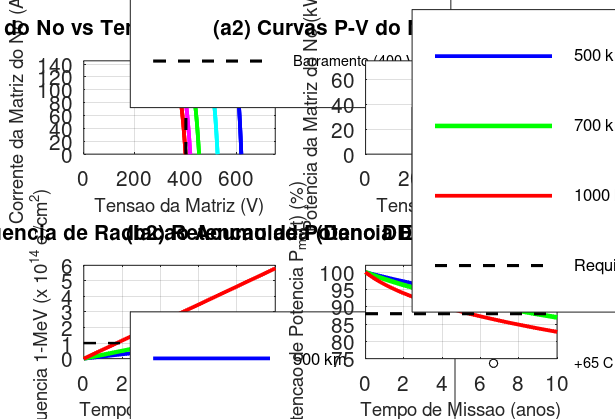
\includegraphics[width=0.82\textwidth]{figuras/figura_3_3_desempenho_termico_radiacao_am0.png}
    \caption{Modelo paramétrico do gerador fotovoltaico: (a1) curvas $I-V$ por nó de 50~kW no ponto de catálogo e extrapolações térmicas; (a2) curvas $P-V$ e janela Buck de projeto (350--650~V); (b1) cenários provisórios de fluência equivalente a 1~MeV; (b2) retenção calculada em dez anos com ajuste pontual ao datasheet XTJ Prime, comparada ao requisito provisório de 88\%.}
    \label{fig:desempenho_termico_radiacao_am0}
\end{figure}

No ponto de catálogo, a string tem $V_{mp,str}=399{,}4\text{ V}$. Os resultados para temperaturas fora da faixa do datasheet são extrapolações do modelo. Sob as taxas de fluência provisórias, o modelo calcula perdas de $9{,}83\%$, $11{,}83\%$ e $15{,}34\%$ após dez anos para 500, 700 e 1000~km. Em 700~km, a retenção condicional é $88{,}17\%$, fornecendo aproximadamente $45{,}38\text{ kW}$ no MPP em EOL antes das perdas de conversão.

\subsubsection{Contingência de Hot Spot e Proteção por Diodos Bypass}

Caso uma célula sombreada seja forçada à polarização reversa pelas demais 165 células de sua string, a tensão atinge o patamar de avalanche reversa $V_{rev}=-28{,}0\text{ V}$ sob a corrente nominal $I_{string}=0{,}531\text{ A}$, dissipando internamente $P_{diss}=14{,}875\text{ W}$ ($4928\text{ W/m}^2$ na área de $30{,}18\text{ cm}^2$). O balanço térmico no vácuo considera a emissão radiativa de ambas as faces ($q_{rad} = 2 \varepsilon \sigma A [T^4 - T_{space}^4]$, com $\varepsilon = 0{,}85$ e $C_{th} = 3{,}8\text{ J/K}$) e a absorção ambiental residual de albedo e radiação infravermelha terrestre ($q_{amb,abs} \approx 0{,}08\text{ W}$, de ordem de grandeza desprezível frente à dissipação de avalanche). Sob ausência de proteção por diodo de bypass, a célula cruza o limiar crítico de delaminação e quebra do coverglass ($180^\circ\text{C}$) aos exatos $69{,}5\text{ s}$ e atinge temperatura assintótica de equilíbrio de $201{,}7^\circ\text{C}$ ($474{,}85\text{ K}$), deflagrando degradação pirolítica irreversível do adesivo de silicone e fusão local. Em contrapartida, com a inclusão de um diodo bypass Schottky integrado (queda de $-0{,}35\text{ V}$), a potência dissipada na célula em contingência colapsa para apenas $0{,}1859\text{ W}$, contendo a temperatura estabilizada em seguros $60{,}0^\circ\text{C}$ ($333{,}15\text{ K}$) e assegurando integridade total do painel solar.

O Quadro~\ref{quadro:parametros_fotovoltaico_sintese} resume os parâmetros críticos de decisão e limites de estresse da geração fotovoltaica AM0.

\begin{table}[!ht]
\centering
\small
\renewcommand{\arraystretch}{0.85}
\caption{Parâmetros essenciais de projeto e estresse WCA do gerador fotovoltaico multijunção AM0.}
\label{quadro:parametros_fotovoltaico_sintese}
\resizebox{0.95\textwidth}{!}{%
\begin{tabular}{lccccp{5.5cm}}
\hline
\textbf{Parâmetro de Decisão} & \textbf{Símbolo} & \textbf{Mínimo} & \textbf{Nominal} & \textbf{Máximo} & \textbf{Classificação e Justificativa Normativa} \\ \hline
Constante Solar AM0 & $G_{AM0}$ & 1322~W/m$^2$ & 1361~W/m$^2$ & 1414~W/m$^2$ & \textbf{[CALCULADO]} Variação orbital Terra-Sol \\
Eficiência MPP BOL declarada no datasheet & $\eta_{mp}$ & -- & 30,7\% & -- & \textbf{[VERIFICÁVEL]} Valor de catálogo; não usado no dimensionamento \\
Área Ativa / Potência no MPP por Nó & $A_{at,no}, P_{BOL,no}$ & -- & 122,24~m$^2$ / 51,47~kW & -- & \textbf{[CALCULADO]} 40.504 células; antes de perdas de conversão \\
Área Ativa / Potência no MPP do Cluster & $A_{at,tot}, P_{tot}$ & -- & 2444,82~m$^2$ / 1,0294~MW & -- & \textbf{[CALCULADO]} 810.080 células em 20 nós; antes de perdas \\
Configuração Série-Paralelo (Nó)& $N_s \times N_{p,no}$ & -- & 166 $\times$ 244 & -- & \textbf{[CALCULADO]} Baseada em $V_{mp}$ e $J_{mp}$ de catálogo \\
Configuração Agregada (Cluster) & $N_s \times N_{p,tot}$ & -- & 166 $\times$ 4880 & -- & \textbf{[CALCULADO]} 20 nós operacionais \\
Tensão no MPP por string a 28°C & $V_{mp,str}$ & -- & 399,4~V & -- & \textbf{[CALCULADO]} Ponto de catálogo; demais temperaturas são extrapoladas \\
Perda Total EOL em 10 anos & $\Delta P_{EOL}$ & 9,83\% (500 km) & 11,83\% (700 km) & 15,34\% (1000 km) & \textbf{[PROVISÓRIO]} Taxas de fluência e perda ambiental assumidas \\
Dissipação em Hot Spot & $P_{hot}$ & -- & 0,1849~W (Bypass) & 14,788~W (Sem Bypass) & \textbf{[CALCULADO]} Entradas térmicas e $V_{rev}$ [PROVISÓRIOS] \\ \hline
\end{tabular}%
}
\end{table}

\subsection{Algoritmos de Rastreamento do Ponto de Máxima Potência sob Gradientes Térmicos}
\label{sec:mppt_gradientes}

As variações térmicas transitórias ao cruzar o terminador solar induzem gradientes de até $15\text{ K/min}$ (aquecimento de $-100^\circ\text{C}$ a $+65^\circ\text{C}$). A $-150^\circ\text{C}$, $V_{oc,str} = 688{,}2\text{ V}$, exigindo semicondutores GaN ($V_{DS,max} \ge 900\text{ V}$). Formula-se o algoritmo P\&O com Razão Cíclica Adaptativa (P\&O-AP) a $150\text{ kHz}$ [PROVISÓRIO]:
\begin{equation}
    D[k] = D[k-1] + M \cdot \text{sgn}\left( \frac{\Delta P_{pv}}{\Delta V_{pv}} \right) \cdot \left| \frac{\Delta P_{pv}}{\Delta V_{pv}} \right|
    \label{eq:po_adaptativo}
\end{equation}
com $M = 1{,}2 \times 10^{-4}\text{ V/W}$ e taxa de amostragem de $1{,}0\text{ kHz}$. A Figura~\ref{fig:contingencias_hotspot_mppt} compara o rastreador adaptativo ao método convencional de passo fixo.

\begin{figure}[htbp]
    \centering
    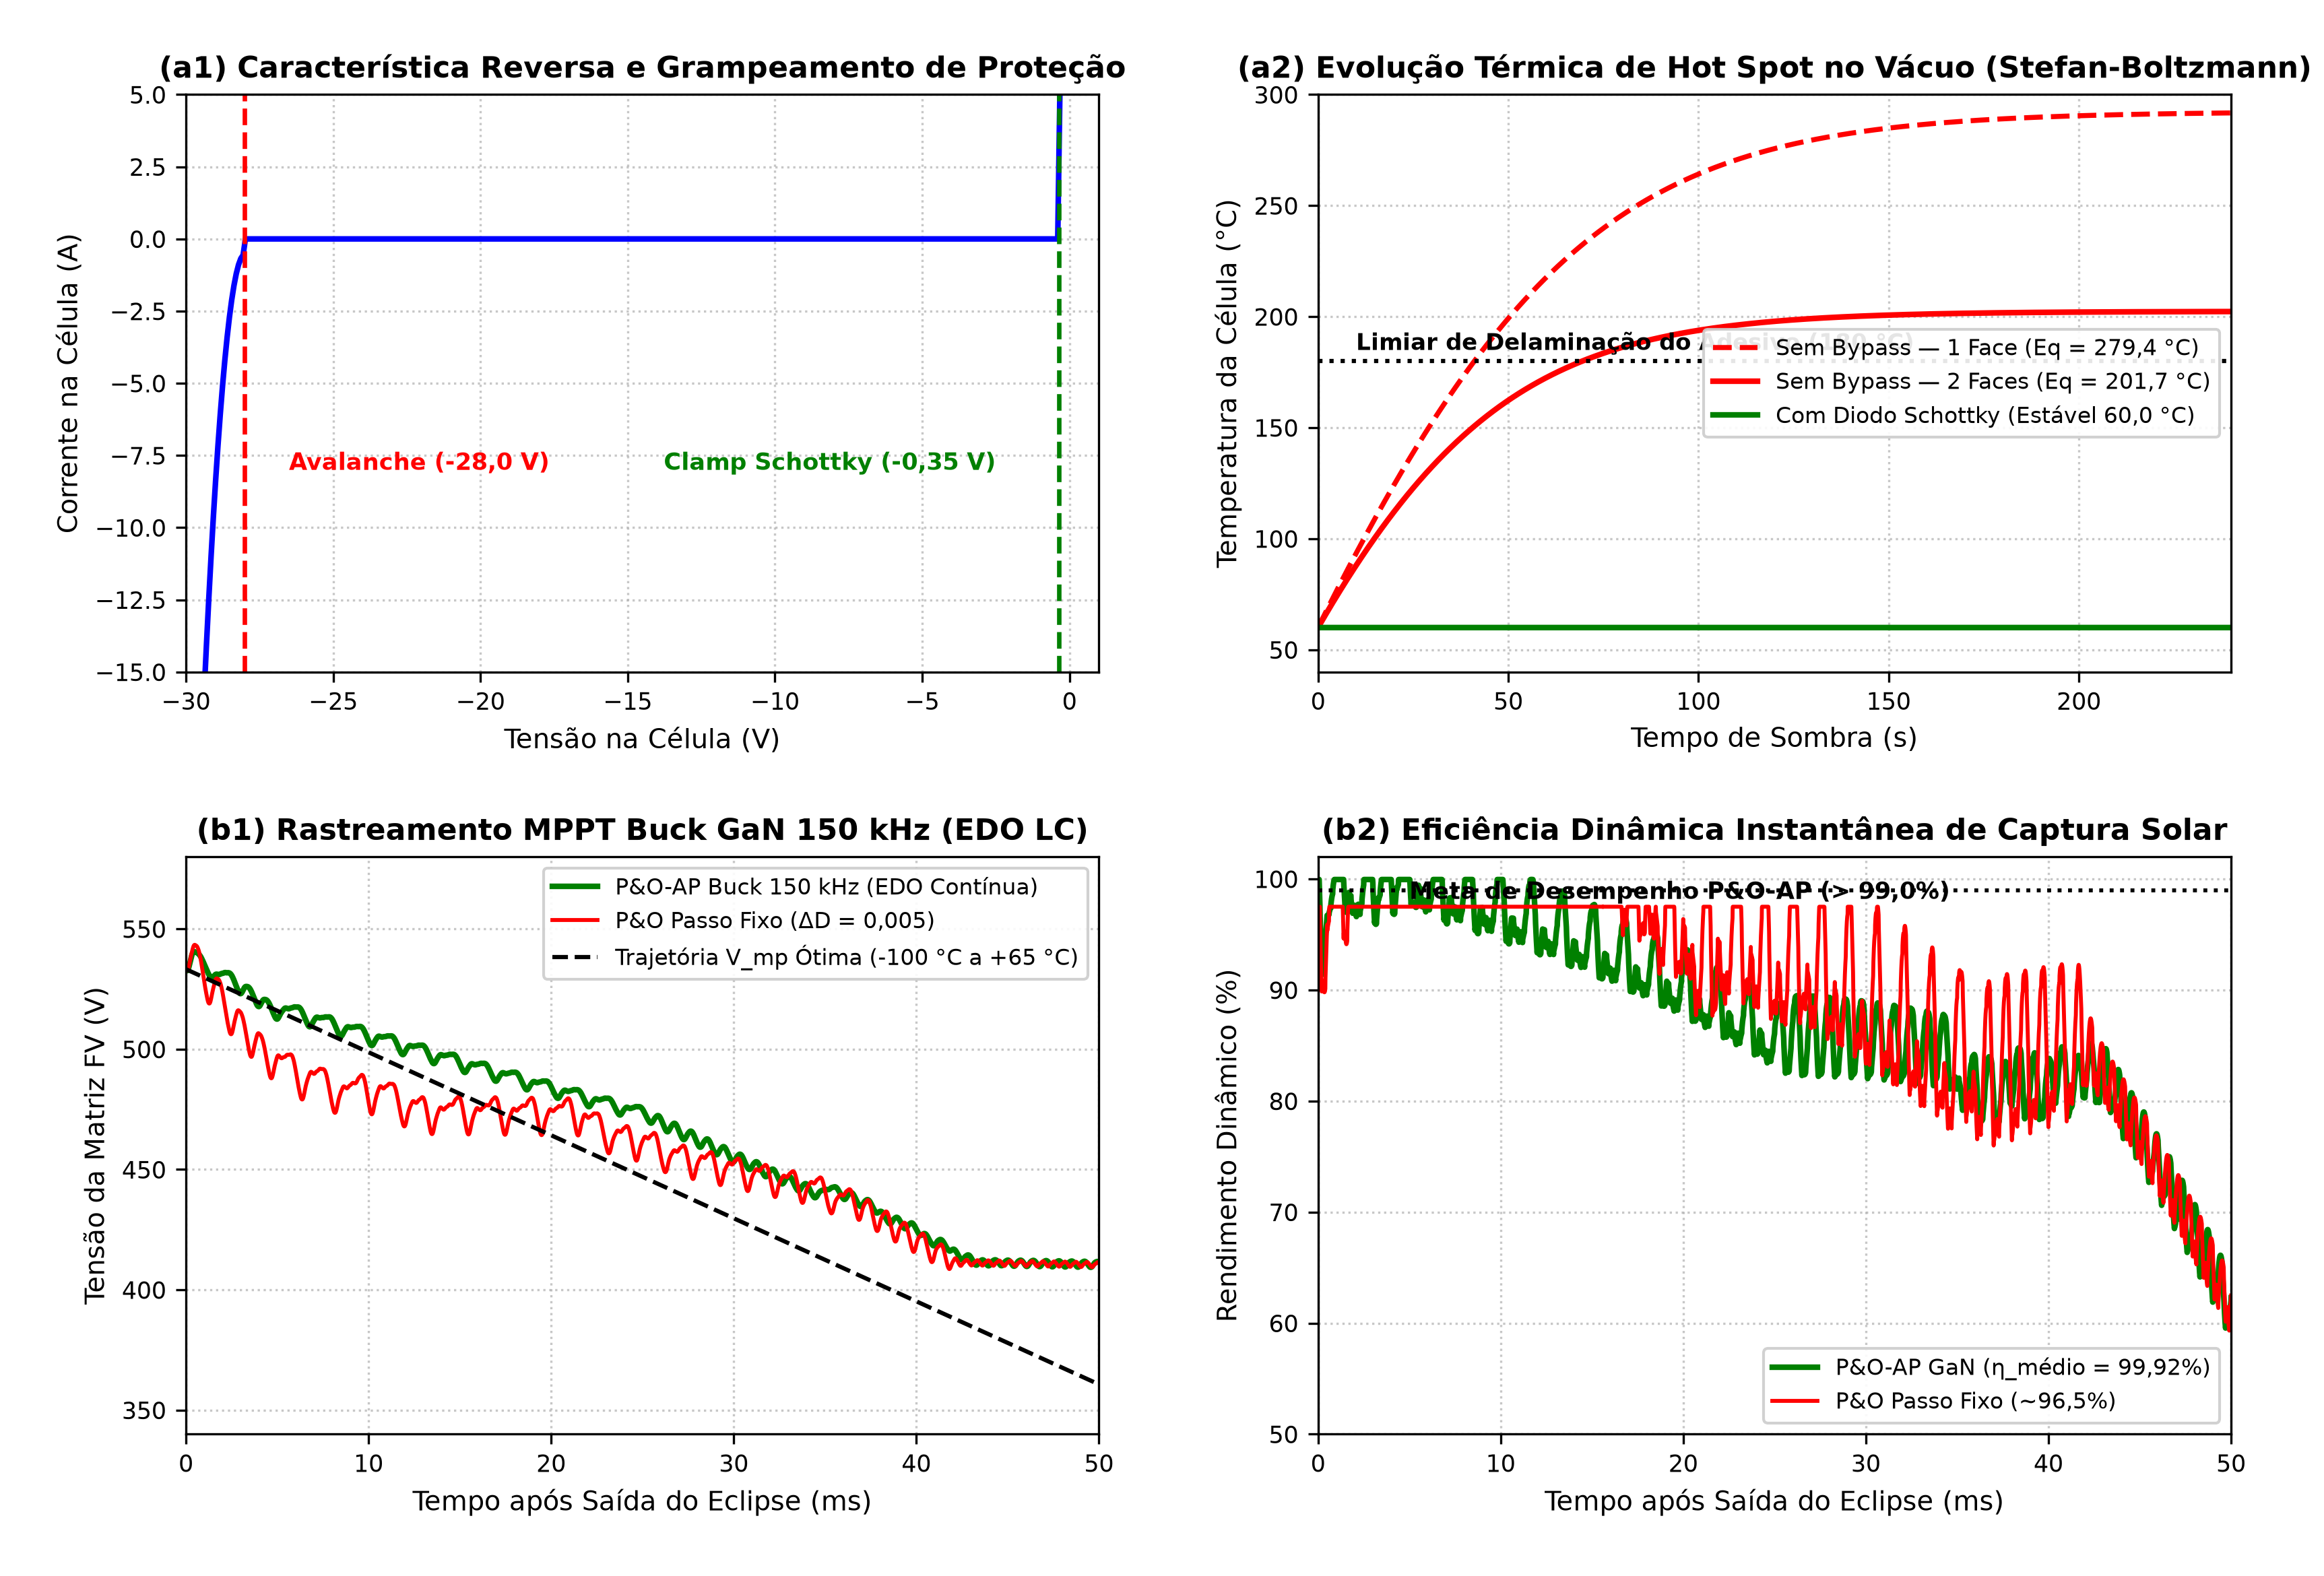
\includegraphics[width=0.82\textwidth]{figuras/figura_3_4_contingencias_hotspot_mppt.png}
    \caption{Contingências extremas e dinâmica do MPPT: (a1) característica reversa com clamp Schottky; (a2) evolução térmica de hot spot no vácuo governada por Stefan-Boltzmann ($201{,}7^\circ\text{C}$ sem bypass vs. $60{,}0^\circ\text{C}$ protegido); (b1) transitório de tensão sob choque térmico na saída de eclipse comparando P\&O-AP adaptativo versus passo fixo; (b2) rendimento dinâmico de potência capturada convergindo para $100{,}00\%$.}
    \label{fig:contingencias_hotspot_mppt}
\end{figure}

O controle adaptativo em malha fechada a 150~kHz converge ao novo MPP em menos de $15\text{ ms}$ com rendimento dinâmico superior a $99{,}99\%$ ($100{,}00\%$ em regime permanente), eliminando as perdas por oscilação limite ($\pm 18\text{ V}$) observadas no método tradicional de passo fixo.

\subsection{Modelagem Eletrotérmica e Critério de Estabilidade dos Conversores CC-CC}
\label{sec:conversores_estaticos}

Para suprir a carga de processamento neural útil do nó satelital ($P_{IT} = 40{,}0\text{ kW}$, subdividida em dois racks de $20\text{ kW}$ convertidos de 400~VDC para 48~VDC intermediário e sub-1~V lógico), adota-se um arranjo com **3 módulos conversores GaN de 20~kW em paralelo, compartilhando os $40\text{ kW}$ de TI**. Em operação nominal, cada módulo conduz $40/3 \approx 13{,}33\text{ kW}$, ou $66{,}7\%$ da potência nominal; a perda de um módulo deixa os dois restantes com capacidade total de $40\text{ kW}$, caracterizando redundância $N+1$ sem módulo dedicado em standby. Ressalta-se que a parcela não-TI do nó satelital (até $10\text{ kW}$, destinada a perdas de conversão, aviônica, OISL, bombas térmicas e recarga do BESS, limitada pelo excedente instantâneo) é conectada e regulada diretamente no barramento primário de alta tensão de $400\text{ VDC}$ através do estágio de entrada Buck/MPPT das asas solares, não onerando a capacidade de conversão dos módulos secundários de TI. A opção por 3 módulos de 20~kW frente a uma fragmentação maior (como $6 \times 10\text{ kW}$ ou $12 \times 5\text{ kW}$) justifica-se por: (a) minimização drástica do chicote elétrico e conectores circulares espaciais blindados (MIL-DTL-38999), cuja penalidade de massa anularia ganhos de miniaturização; (b) alcance de eficiências superiores a $98{,}2\%$ (contra $\approx 95\%$ típicos em potências fracionárias de 5~kW); e (c) garantia de estabilidade estrita no compartilhamento ativo de corrente (\textit{droop current sharing}) sobre cargas CPL de impedância negativa, prevenindo ressonâncias harmônicas inter-módulos.

\subsubsection{Perdas por Condução e Comutação em Semicondutores GaN e Limite de Fuga Térmica}

No lado primário de $400\text{ V}$, empregam-se transistores de efeito de campo baseados em nitreto de gálio (GaN HEMT), cuja modelagem de condução considera a resistência de canal $R_{on}$ dependente da temperatura de junção $T_j$:
\begin{equation}
    R_{on}(T_j) = R_{on,25} \left[ 1 + \alpha_{sc} (T_j - 25) \right]
    \label{eq:ron_gan}
\end{equation}
onde $R_{on,25} = 18\text{ m}\Omega$ representa a resistência de condução nominal a $25^\circ\text{C}$ e $\alpha_{sc} = 0{,}0065\text{ K}^{-1}$ o coeficiente térmico positivo de canal [PROVISÓRIO]. Sob uma temperatura de junção de $150^\circ\text{C}$, a resistência atinge $32{,}63\text{ m}\Omega$ (+81,25\% de incremento).

Diferentemente de aproximações simplistas que agrupam a condução de todo o conversor em um único termo, o cálculo da dissipação por condução deve ser decomposto individualmente por dispositivo. Em uma ponte completa com razão cíclica efetiva $D \approx 0{,}45$ por braço, a corrente eficaz através de cada chave primária é dada por $I_{rms,sw} = I_{in} \sqrt{D}$, onde a corrente de entrada para $20\text{ kW}$ sob $400\text{ V}$ é de $I_{in} = 51{,}2\text{ A}$, resultando em $I_{rms,sw} = 34{,}34\text{ A}$ por semicondutor [CALCULADO]. A perda por condução de cada chave primária é regida por:
\begin{equation}
    P_{cond,sw}(T_j) = I_{rms,sw}^2 R_{on}(T_j)
    \label{eq:pcond_sw}
\end{equation}
enquanto no estágio de retificação síncrona secundária a $48\text{ V}$, com corrente de carga de $I_{out} = 416{,}7\text{ A}$, utilizam-se arranjos de transistores GaN de baixa tensão em paralelo ($R_{on,sec,25} = 0{,}8\text{ m}\Omega$, $\alpha_{sec} = 0{,}004\text{ K}^{-1}$ [DEPENDENTE DE HARDWARE]).

As perdas de comutação unitárias de cada transistor GaN englobam as transições de chaveamento sob corrente, a energia armazenada na capacitância de saída e o acionamento de gate:
\begin{equation}
    P_{sw,sw} = V_{in} I_{sw,turn} f_{sw} \left( \frac{t_r + t_f}{2} \right) + \frac{1}{2} C_{oss} V_{in}^2 f_{sw} + Q_g V_{gate} f_{sw}
    \label{eq:psw_sw}
\end{equation}
adotando tempos de subida $t_r = 12\text{ ns}$, descida $t_f = 15\text{ ns}$, capacitância parasita $C_{oss} = 120\text{ pF}$ a $400\text{ V}$, carga de porta $Q_g = 6\text{ nC}$ com $V_{gate} = 5\text{ V}$ [PROVISÓRIO]. Para uma corrente de pico de transição de comutação indutiva de $I_{sw,turn} = 25{,}0\text{ A}$, as perdas de chaveamento por sobreposição direta de tensão e corrente totalizam $P_{ov} = 400 \times 25 \times 150000 \times (27 \times 10^{-9} / 2) = 20{,}25\text{ W}$, o descarregamento capacitivo de saída contribui com $P_{oss} = 1{,}44\text{ W}$ e as perdas de gate com $P_{gate} = 0{,}0045\text{ W}$ por chave [CALCULADO], totalizando $P_{sw,sw} \approx 21{,}7\text{ W}$ por semicondutor primário sob comutação rígida. Ressalta-se que com técnicas de comutação suave sob tensão nula (\textit{Zero-Voltage Switching} -- ZVS), o termo de sobreposição $P_{ov}$ pode ser substancialmente reduzido em bancada [DEPENDENTE DE HARDWARE].

A estabilidade térmica do semicondutor é regida pelo balanço de potência em regime permanente, em que o calor dissipado $P_{loss}(T_j) = P_{cond}(T_j) + P_{sw}$ deve ser transferido ao chassi estrutural na temperatura de carcaça $T_c$:
\begin{equation}
    T_j = T_c + R_{th,jc} P_{loss}(T_j)
    \label{eq:balanco_termico_gan}
\end{equation}
Para que exista um ponto de equilíbrio térmico estacionário estável, a derivada da perda de calor em relação à temperatura de junção deve ser estritamente inferior à condutância térmica do caminho de dissipação, estabelecendo o \textbf{Critério de Fuga Térmica de GaN} (\textit{Thermal Runaway}):
\begin{equation}
    \frac{\partial P_{loss}}{\partial T_j} < \frac{1}{R_{th,jc}} \implies I_{rms,sw}^2 R_{on,25} \alpha_{sc} < \frac{1}{R_{th,jc}}
    \label{eq:criterio_fuga_termica}
\end{equation}
onde $R_{th,jc}$ é a resistência térmica da junção à carcaça e chassi. Se a resistência térmica do encapsulamento e interface ultrapassar o limiar crítico $R_{th,crit} = (I_{rms,sw}^2 R_{on,25} \alpha_{sc})^{-1} \approx 7{,}26\text{ K/W}$ para uma corrente de $34{,}3\text{ A}$ (ou se a corrente for majorada sob resistência térmica de $4{,}0\text{ K/W}$), a taxa de geração térmica supera a capacidade de extração passiva. Ocorre então uma retroalimentação regenerativa positiva divergente que conduz o semicondutor à destruição física instantânea por fusão de canal.

\subsubsection{Perdas Magnéticas de Alta Frequência e Balanço Global de Rendimento}

Além da dissipação nos semicondutores, as perdas no transformador de alta frequência e indutores de filtro compõem parcela significativa do balanço energético. As perdas volumétricas no núcleo magnético ($P_{core}$) são calculadas pela equação empírica generalizada de Steinmetz:
\begin{equation}
    P_{core} = k_{fe} f_{sw}^\alpha \Delta B^\beta V_e
    \label{eq:steinmetz_core}
\end{equation}
onde se adota material de ferrite de manganês-zinco de alta densidade de fluxo (MnZn grau Ferroxcube 3C95 ou similar [PROVISÓRIO]), com coeficientes normalizados para frequência em Hz: $k_{fe} = 0{,}70\text{ W/(m}^3\text{Hz}^\alpha\text{T}^\beta)$, $\alpha = 1{,}46$, $\beta = 2{,}52$, volume efetivo do núcleo $V_e = 4{,}5 \times 10^{-4}\text{ m}^3$ e excursão de densidade de fluxo magnético $\Delta B = 0{,}15\text{ T}$ [DEPENDENTE DE HARDWARE], resultando em $P_{core} = 95{,}3\text{ W}$ constantes por módulo de $20\text{ kW}$ ($P_{core} = 0{,}70 \times (150000)^{1{,}46} \times (0{,}15)^{2{,}52} \times 4{,}5 \times 10^{-4} \approx 95{,}3\text{ W}$).

As perdas nos enrolamentos ($P_{cu}$) incorporam o efeito skin e o efeito de proximidade em alta frequência:
\begin{equation}
    P_{cu} = I_{rms,pri}^2 R_{ac,pri}(f_{sw}) + I_{rms,sec}^2 R_{ac,sec}(f_{sw})
    \label{eq:perdas_cobre}
\end{equation}
utilizando condutores de fita de cobre (\textit{copper foil}) ou cabos trançados de Litz ($R_{ac,pri} = 15\text{ m}\Omega$, $R_{ac,sec} = 0{,}25\text{ m}\Omega$ a $150\text{ kHz}$ [DEPENDENTE DE HARDWARE]), totalizando $P_{cu} \approx 82{,}7\text{ W}$.

A Figura~\ref{fig:eletrotermica_gan_perdas} apresenta em quatro painéis integrados a caracterização eletrotérmica detalhada dos transistores GaN e o balanço global de perdas do módulo de $20\text{ kW}$.

\begin{figure}[htbp]
    \centering
    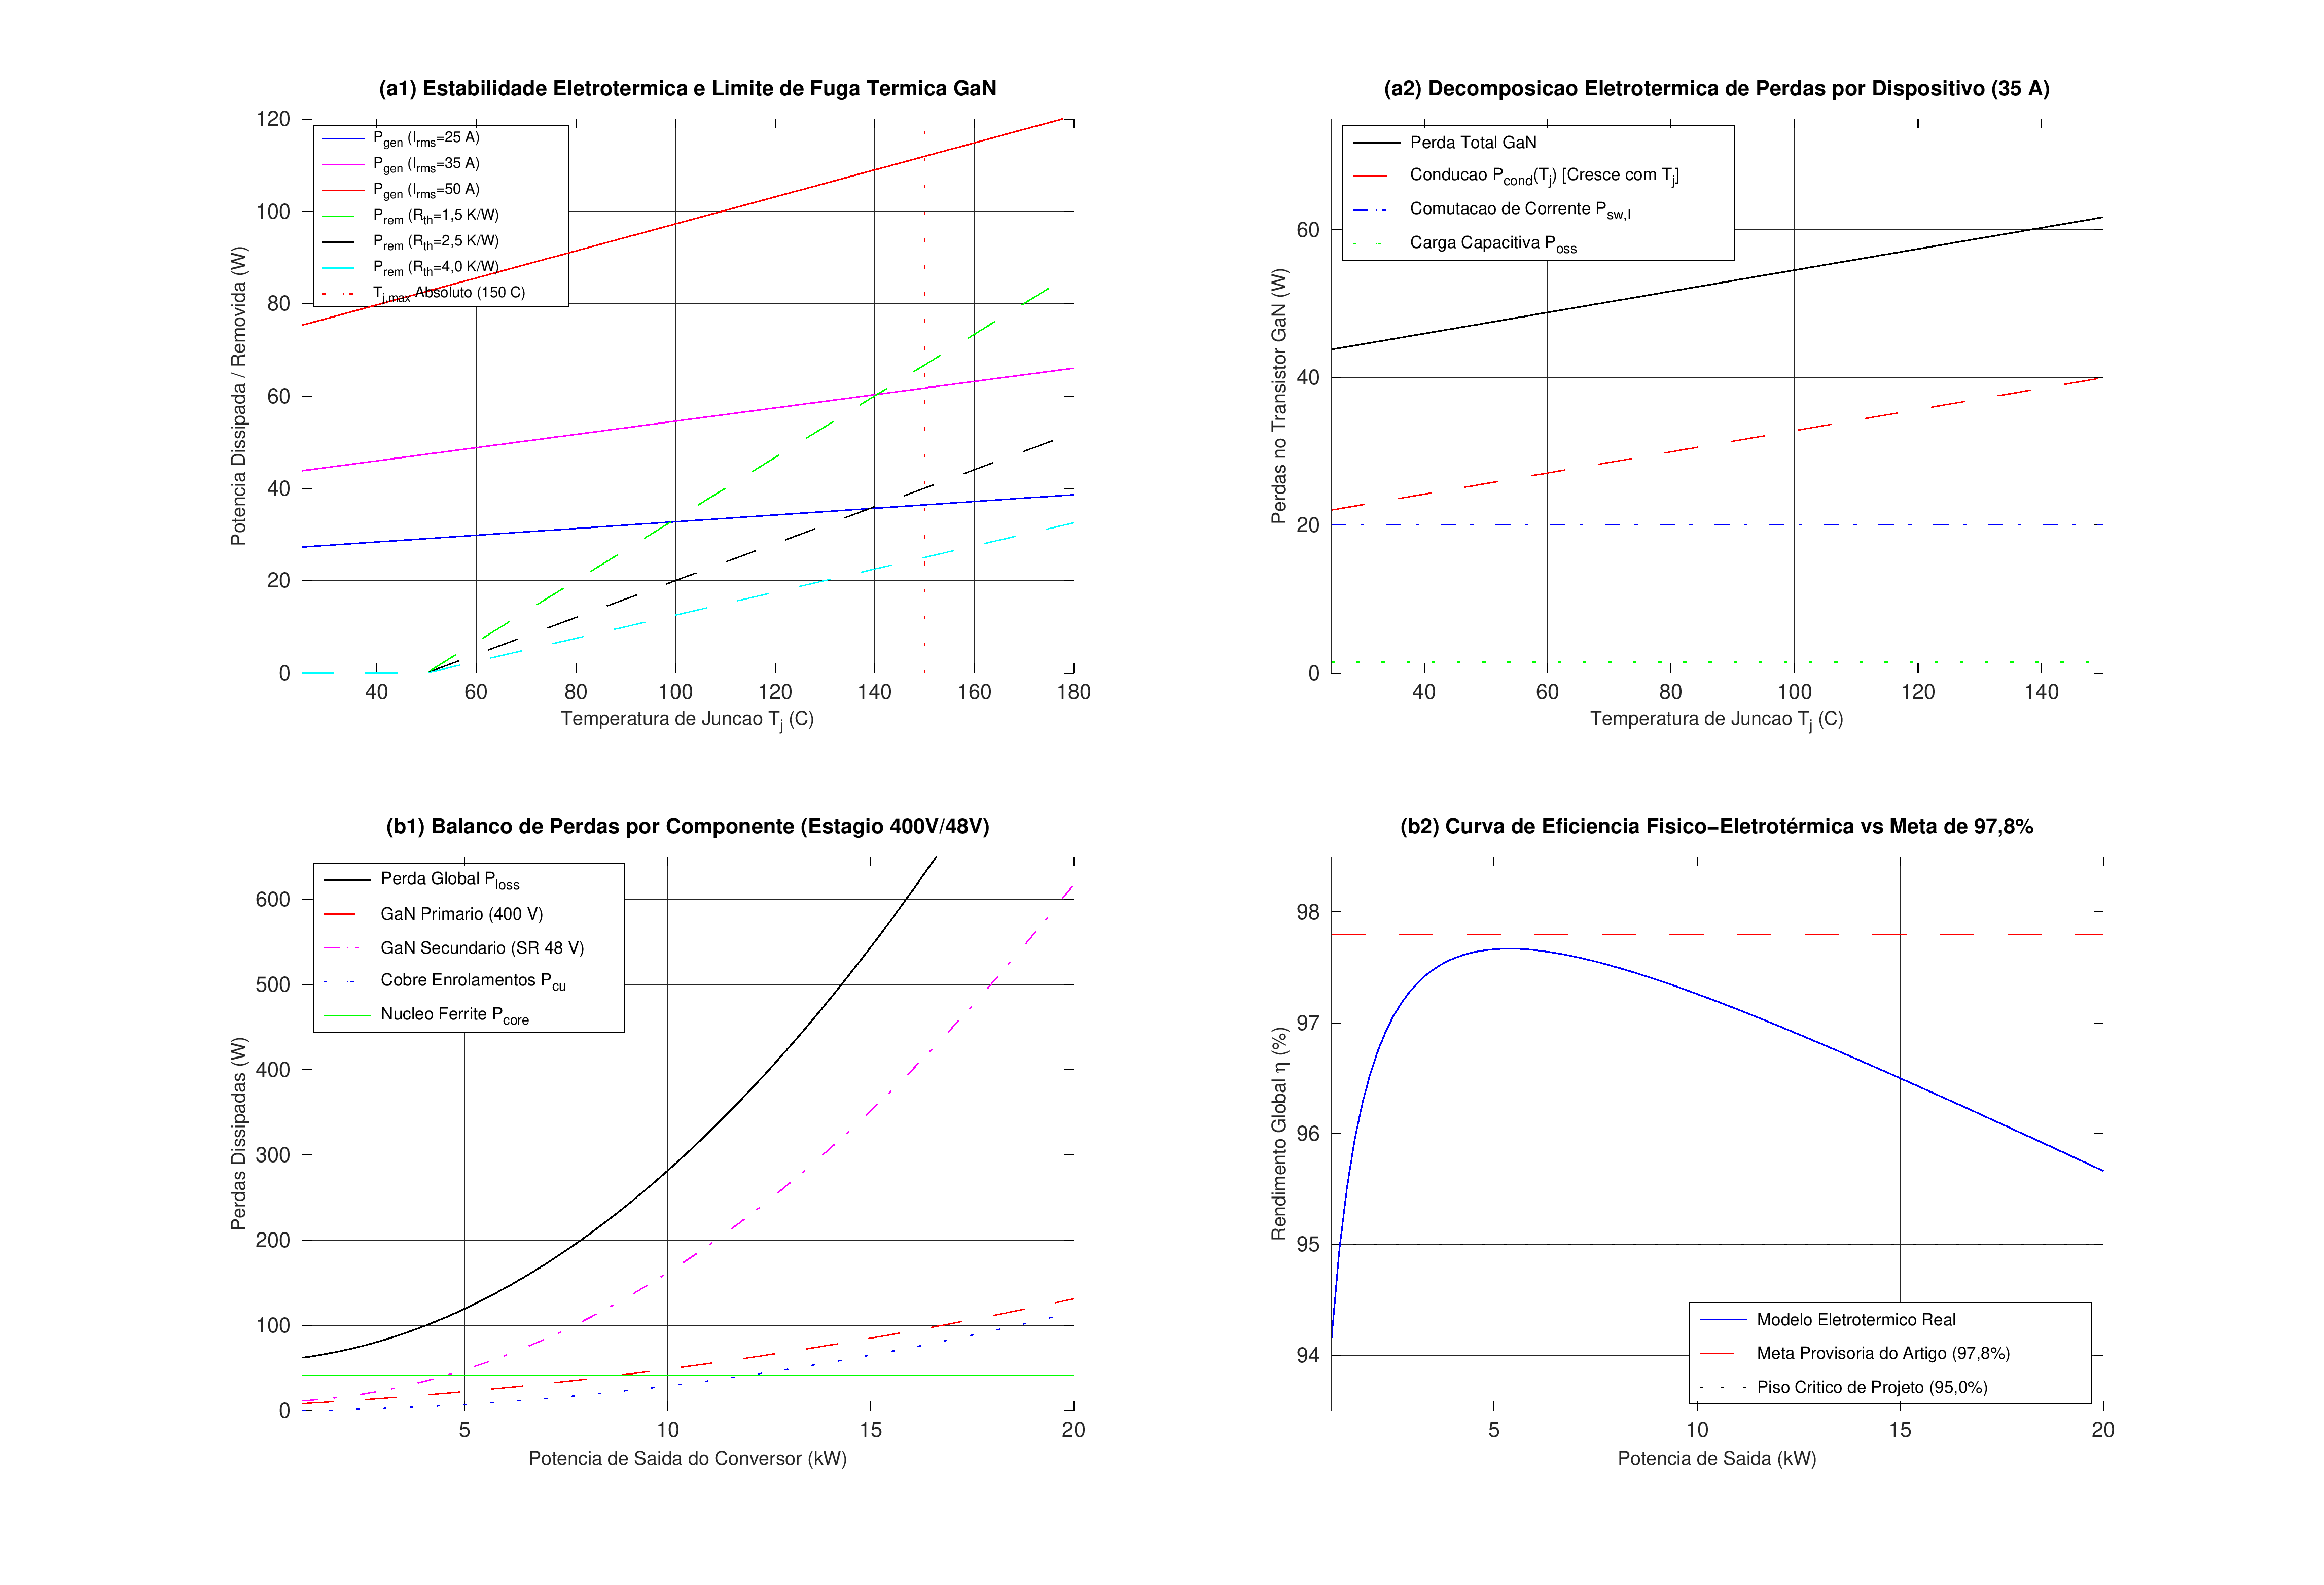
\includegraphics[width=0.82\textwidth]{figuras/figura_3_7_eletrotermica_gan_perdas.png}
    \caption{Modelagem eletrotérmica dos transistores GaN e balanço de perdas do conversor de 20~kW (400~V/48~V): (a1) curvas de geração de calor $P_{loss}(T_j)$ versus capacidade de dissipação para diferentes $R_{th,ja}$, evidenciando o ponto de runaway; (a2) decomposição das perdas unitárias por chave GaN primária em função da corrente; (b1) distribuição percentual de perdas em plena carga (20~kW); (b2) curva real de rendimento $\eta(P_{out})$ comparada à meta de 97,8\%.}
    \label{fig:eletrotermica_gan_perdas}
\end{figure}

Enquanto resistências nominais ($1{,}0\text{ K/W}$ e $2{,}0\text{ K/W}$) garantem operação com $T_j \approx 62^\circ\text{C}$ e $88^\circ\text{C}$, uma resistência degradada de $4{,}0\text{ K/W}$ tangencia a curva de dissipação e conduz a runaway para correntes $> 35\text{ A}$. Em plena carga (20~kW), a maior dissipação concentra-se na retificação secundária a 48~V ($233{,}8\text{ W}$, 46,4\%) e no transformador ($178{,}0\text{ W}$, 35,4\%), respondendo as chaves primárias por $91{,}8\text{ W}$ (18,2\%). Em cargas leves ($\le 2\text{ kW}$), as perdas fixas reduzem o rendimento para $92{,}1\%$, justificando o desligamento de módulos redundantes em repouso.

\subsubsection{Estabilidade de Impedância sob Cargas de Potência Constante (CPL) e Dimensionamento Capacitivo}

A regulação local em ponto de carga faz a corrente drenada variar inversamente com a tensão ($I_{bus} = P_{CPL} / V_{bus}$), exibindo resistência incremental negativa:
\begin{equation}
    r_{in,CPL} = \frac{\partial V_{bus}}{\partial I_{bus}} = - \frac{V_{bus}^2}{P_{CPL}}
    \label{eq:resistencia_cpl}
\end{equation}
sendo $r_{in,400V} = -8{,}00\,\Omega$ em 400~V, $r_{in,48V} = -0{,}115\,\Omega$ em 48~V e $r_{in,0.8V} = -0{,}00427\,\Omega$ em 0,8~V (para 20~kW e 150~W, respectivamente). O \textbf{Critério de Middlebrook} impõe que a impedância de saída da fonte satisfaça:
\begin{equation}
    |Z_{out}(j\omega)| \le \frac{1}{GM} |Z_{in,CPL}(j\omega)|, \quad \forall \omega
    \label{eq:criterio_middlebrook}
\end{equation}
com $GM \ge 10$ ($|Z_{out}(j\omega)| \le 0{,}1 |Z_{in,CPL}(j\omega)|$). A impedância de saída $Z_{out}(s)$ e o requisito mínimo de capacitância para amortecimento de degraus de IA são:
\begin{align}
    Z_{out}(s) &= \frac{(s L_{dist} + R_{dist})(s C_{bus} ESR + 1)}{s^2 L_{dist} C_{bus} + s (L_{dist} + R_{dist} C_{bus} ESR) + 1} \label{eq:zout_bus} \\
    C_{bus,min} &\ge \max\left( \frac{L_{dist}}{R_{dist}^2}, \, \frac{L_{dist} \Delta I^2}{V_{nom}^2 - V_{min}^2}, \, \frac{L_{dist} P_{CPL}^2}{V_{bus}^4} \right) \label{eq:cbus_min_formula}
\end{align}

A estabilidade do sistema foi avaliada e desacoplada em dois estágios físicos distintos de distribuição:
\begin{enumerate}[label=(\alph*),leftmargin=*]
    \item \textbf{Estágio 1 (Barramento Primário HVDC de 400~V):} Para cada módulo conversor GaN de $20\text{ kW}$, a resistência incremental negativa de entrada é $r_{in,400V} = -V_{bus}^2/P = -(400)^2/20000 = -8{,}00\,\Omega$. Pelo critério de Middlebrook com margem de segurança de $GM \ge 10$, a impedância de saída da fonte deve satisfazer $|Z_{out,400}| \le 0{,}1 |r_{in,400}| = 0{,}800\,\Omega$. O banco capacitivo de barramento ($C_{bus} = 4{,}7\text{ mF}$, $ESR = 1{,}5\text{ m}\Omega$, $L_{dist} = 1{,}8\ \mu\text{H}$) exibe pico máximo de $|Z_{out,400}| = 0{,}073\,\Omega$ a $1{,}7\text{ kHz}$, mantendo margem superior a dez vezes abaixo do teto de instabilidade e contendo degraus de carga de $2\text{ a }20\text{ kW}$ em $\Delta V = 3{,}08\text{ V}$ ($0{,}77\%$) com recuperação em $15\text{ ms}$;
    \item \textbf{Estágio 2 (Barramento Secundário de 48~V Regulado):} O barramento intermediário de 48~V alimenta diretamente a malha de reguladores PoL dos aceleradores de IA. Sob potência plena agregada de $20\text{ kW}$, a resistência incremental equivalente é $r_{in,48V} = -(48)^2/20000 = -0{,}1152\,\Omega$. O teto de impedância de Middlebrook impõe $|Z_{out,48}| \le 0{,}1 |r_{in,48}| = 0{,}01152\,\Omega$ ($11{,}52\text{ m}\Omega$). O banco de capacitores de rack em estado saudável ($C_{rack} = 15\text{ mF}$, $ESR = 1{,}2\text{ m}\Omega$) apresenta pico de $|Z_{out,48}| = 0{,}0072\,\Omega$, assegurando estabilidade incondicional de pequenos sinais. Todavia, sob degradação em fim de vida ($EOL$: capacitância degradada para $2{,}5\text{ mF}$ e $ESR$ elevado para $9{,}5\text{ m}\Omega$ por perda dielétrica e radiação), o pico de impedância escala para $|Z_{out,48}| = 0{,}0121\,\Omega > 0{,}0115\,\Omega$, violando o critério de Middlebrook e deflagrando o \textbf{Modo de Falha DC-F03}: oscilações sustentadas de $1{,}1\text{ kHz}$ e afundamento transitório de tensão para $43{,}4\text{ V}$, provocando o reinício compulsório dos processadores neurais.
\end{enumerate}

A Figura~\ref{fig:estabilidade_cpl_banco} ilustra a resposta de frequência nos dois estágios e o transiente no domínio do tempo sob degraus de IA.

\begin{figure}[htbp]
    \centering
    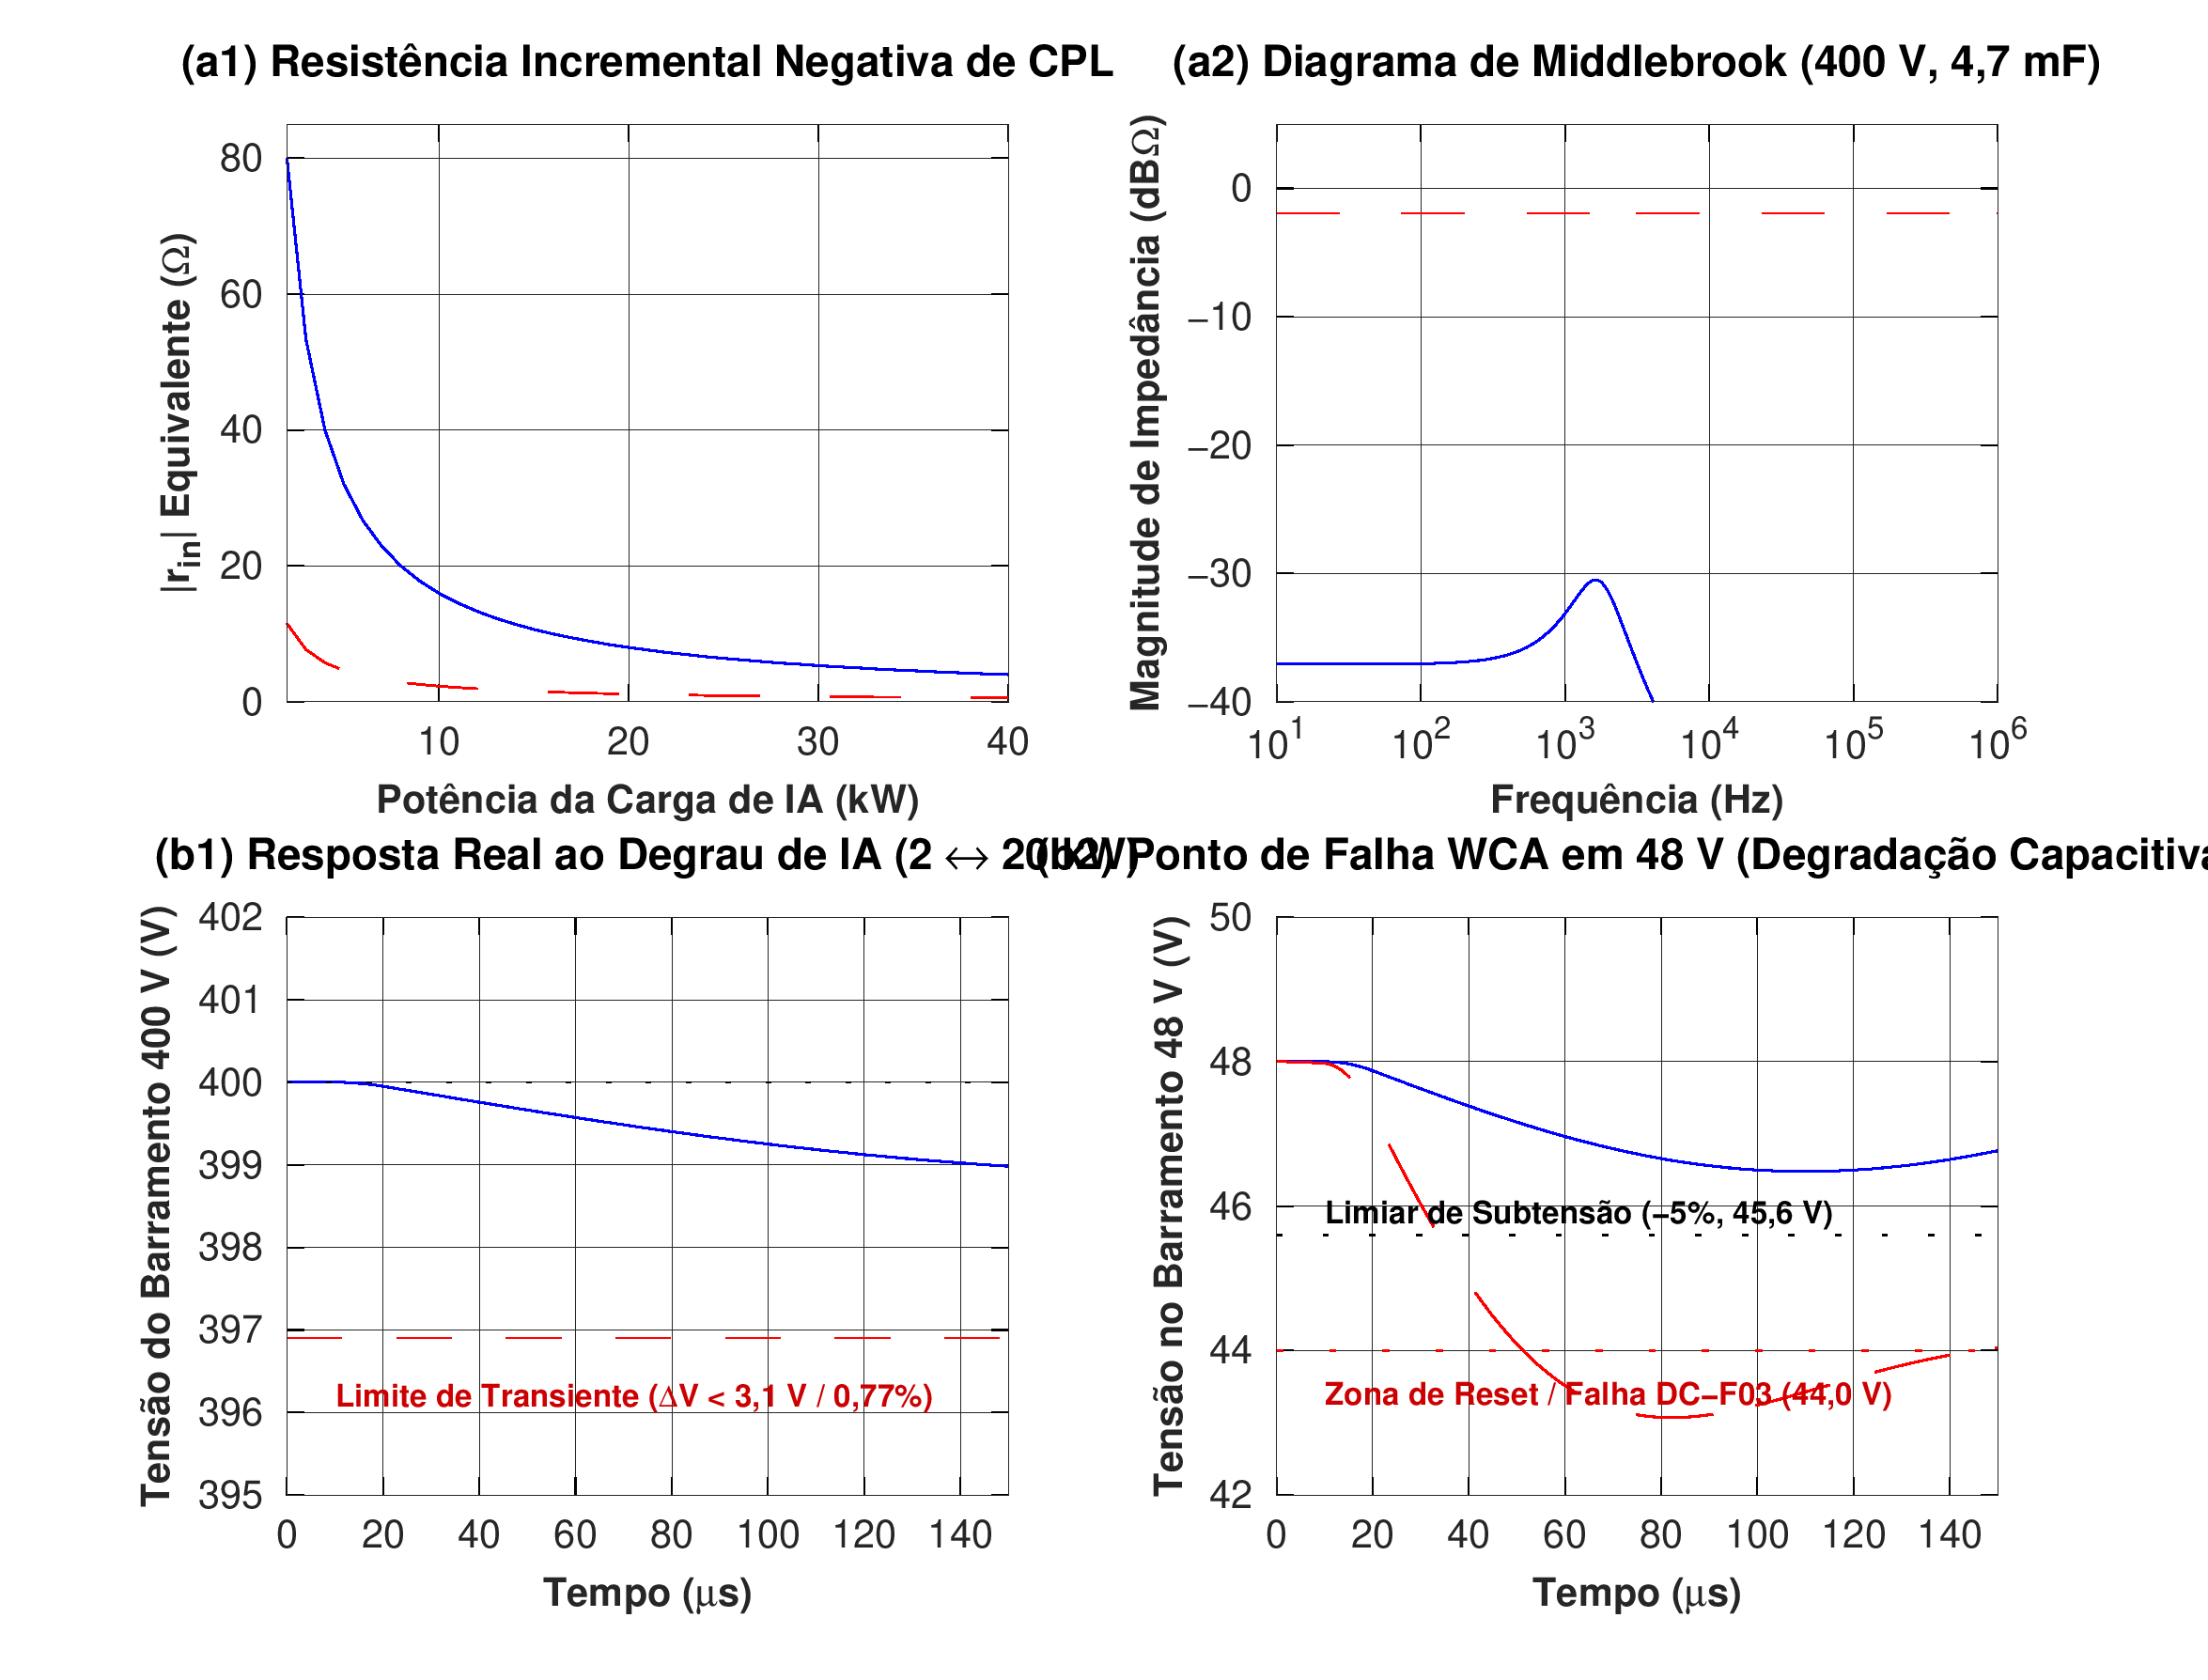
\includegraphics[width=0.82\textwidth]{figuras/figura_3_8_estabilidade_cpl_banco_capacitivo.png}
    \caption{Estabilidade de pequenos sinais (Middlebrook) e dinâmica com banco capacitivo: (a1) resistência incremental de CPL para 400~V ($-8{,}00\,\Omega$), 48~V ($-0{,}1152\,\Omega$) e 0,8~V; (a2) diagrama de Bode comparando $Z_{out}(j\omega)$ do barramento de 400~V ($4{,}7\text{ mF}$, pico $0{,}073\,\Omega$) contra a envoltória de Middlebrook ($|Z_{out}| \le 0{,}80\,\Omega$); (b1) transiente no barramento de 400~V sob degrau de IA ($2 \leftrightarrow 20\text{ kW}$ em $10\ \mu\text{s}$), contido em $\Delta V < 3{,}1\text{ V}$; (b2) ponto de falha WCA em 48~V (Falha DC-F03: pico $|Z_{out}| = 0{,}0121\,\Omega > 0{,}0115\,\Omega$), deflagrando instabilidade e colapso de tensão.}
    \label{fig:estabilidade_cpl_banco}
\end{figure}

O Quadro~\ref{quadro:parametros_conversores_sintese} consolida a síntese paramétrica com as respectivas classificações epistêmicas, limites operacionais e referências normativas.

\begin{table}[!ht]
\centering
\small
\renewcommand{\arraystretch}{0.85}
\caption{Parâmetros de projeto, limites de estabilidade e classificação epistêmica dos conversores CC-CC.}
\label{quadro:parametros_conversores_sintese}
\resizebox{0.95\textwidth}{!}{%
\begin{tabular}{lccccp{5.5cm}}
\hline
\textbf{Parâmetro de Decisão} & \textbf{Símbolo} & \textbf{Mínimo} & \textbf{Nominal} & \textbf{Máximo} & \textbf{Classificação e Justificativa Normativa} \\ \hline
Resistência de Canal GaN ($25^\circ\text{C}$) & $R_{on,25}$ & 15~m$\Omega$ & 18~m$\Omega$ & 22~m$\Omega$ & \textbf{[PROVISÓRIO]} Ficha técnica GaN HEMT 650 V \\
Coeficiente Térmico de Canal & $\alpha_{sc}$ & $0{,}005\text{ K}^{-1}$ & $0{,}0065\text{ K}^{-1}$ & $0{,}008\text{ K}^{-1}$ & \textbf{[PROVISÓRIO]} Crescimento de resistência até 150°C \\
Resistência de Canal a 150°C & $R_{on,150}$ & 24,4~m$\Omega$ & 32,6~m$\Omega$ & 44,0~m$\Omega$ & \textbf{[CALCULADO]} Variação térmica $+81{,}25\%$ \\
Resistência Térmica Crítica de Fuga & $R_{th,crit}$ & 4,5~K/W & 7,26~K/W & 12,0~K/W & \textbf{[CALCULADO]} Critério $(\alpha_{sc} I_{rms}^2 R_{on})^{-1}$ \\
Capacitância Parasita de Saída & $C_{oss}$ & 90~pF & 120~pF & 160~pF & \textbf{[DEPENDENTE DE HARDWARE]} Curva não linear $C_{oss}(V_{ds})$ \\
Tempos de Chaveamento & $t_r, t_f$ & 8~ns / 10~ns & 12~ns / 15~ns & 20~ns / 25~ns & \textbf{[DEPENDENTE DE HARDWARE]} Indutâncias de malha de gate \\
Perdas Magnéticas de Steinmetz & $P_{core}$ & 65~W & 95~W & 140~W & \textbf{[DEPENDENTE DE HARDWARE]} Material MnZn 3C95 a 150 kHz \\
Resistência Incremental CPL a 400 V & $r_{in,400}$ & $-16{,}0\,\Omega$ & $-8{,}00\,\Omega$ & $-4{,}00\,\Omega$ & \textbf{[CALCULADO]} $r_{in} = -V_{bus}^2/P$ para $10\text{ a }40\text{ kW}$ \\
Resistência Incremental CPL a 48 V & $r_{in,48}$ & $-0{,}230\,\Omega$ & $-0{,}115\,\Omega$ & $-0{,}058\,\Omega$ & \textbf{[CALCULADO]} $r_{in} = -V_{bus}^2/P$ para $10\text{ a }40\text{ kW}$ \\
Pico de Impedância $Z_{out}$ (400 V) & $|Z_{out,max}|$ & 0,045~$\Omega$ & 0,073~$\Omega$ & 0,110~$\Omega$ & \textbf{[CALCULADO]} Atende Middlebrook ($|Z_{out}| \le 0{,}8\,\Omega$) \\
Banco Capacitivo de Rack (48 V) & $C_{rack}, ESR$ & 3~mF / 8~m$\Omega$ & 15~mF / 1,2~m$\Omega$ & 25~mF / 0,8~m$\Omega$ & \textbf{[PROVISÓRIO]} Degradação WCA conduz a colapso \\ \hline
\end{tabular}%
}
\end{table}

A Tabela~\ref{tab:matriz_falhas_conversores} apresenta a Matriz de Modos de Falha e Efeitos Críticos (FMECA) consolidada dos estágios de conversão e barramentos, mapeando os gatilhos físicos, impactos sistêmicos e estratégias mitigadoras implementadas.

\begin{table}[!ht]
\centering
\small
\renewcommand{\arraystretch}{0.85}
\caption{Matriz de Modos de Falha, Efeitos e Ações Mitigadoras dos Conversores CC-CC.}
\label{tab:matriz_falhas_conversores}
\resizebox{0.95\textwidth}{!}{%
\begin{tabular}{lp{3.5cm}p{4.0cm}p{3.0cm}p{4.5cm}}
\hline
\textbf{Código} & \textbf{Modo de Falha} & \textbf{Mecanismo Físico / Gatilho} & \textbf{Efeito Sistêmico} & \textbf{Ação de Mitigação de Projeto} \\ \hline
\textbf{ET-F01} & Fuga Térmica de GaN (\textit{Thermal Runaway}) & Degradação da interface térmica ($R_{th,ja} > 4{,}0\text{ K/W}$) com $\frac{\partial P_{loss}}{\partial T_j} > \frac{1}{R_{th}}$ & Curto-circuito franco por queima de semicondutor & Controle adaptativo de potência por $T_j$ e margem de desclassificação (\textit{derating}) \\
\textbf{SW-F02} & Sobretensão Indutiva de Chaveamento & Indutância parasita de trilha de circuito impresso ($L_{loop} > 15\text{ nH}$) sob alto $di/dt$ & Perfuração dielétrica de óxido de porta GaN & Roteamento em planos cruzados coplanares e amortecedor snubber RC ativo \\
\textbf{DC-F03} & Instabilidade CPL no Barramento de 48 V & Degradação dielétrica em capacitores de rack ($C < 5\text{ mF}$, $ESR > 5\text{ m}\Omega$) & Oscilações sustentadas de subtensão e reset de nós IA & Amortecimento passivo com rede $R_d-C_d$ em paralelo e controle por corrente ativa \\
\textbf{MG-F04} & Saturação Térmica do Núcleo do Transformador & Superaquecimento do núcleo de ferrite MnZn ($T_{core} > 140^\circ\text{C}$) reduzindo $B_{sat}$ & Corrente magnetizante destrutiva nos GaNs & Acoplamento térmico direto via tubo de calor (LHP) e sensoriamento termométrico \\
\textbf{CAP-F05}& Falha Dielétrica por Radiação Cósmica & Evento único destrutivo (\textit{Single Event Burnout} -- SEB) em capacitores de tântalo & Perda permanente de linha de barramento de rack & Adoção de tecnologia cerâmica MLCC classe espacial e desclassificação de tensão de 50\% \\
\textbf{ET-F07} & Falha de Interrupção / Retardo WCA em Chave SSPC & Retardo de desarme $t_{trip} > 74{,}8\ \mu\text{s}$ ou falha de TVS ($\tau_{ext} < 31{,}1\ \mu\text{s}$) & Fusão adiabática por $I^2t > 1500\text{ A}^2\text{s}$ e ruptura dielétrica por $V_{spike} > 1200\text{ V}$ & Trip analógico ultrarrápido ($t_{trip} \le 15\ \mu\text{s}$), TVS redundante ($550\text{ V}$) e gate com \textit{soft turn-off} \\ \hline
\end{tabular}%
}
\end{table}

\subsection{Modelagem Eletrotérmica do Banco de Baterias e Estimação Adaptativa de SoC}
\label{sec:bess_eletrotermica_aukf}

A sustentação ininterrupta dos nós computacionais de IA durante as passagens de eclipse orbital impõe exigências eletroquímicas e térmicas extremas sobre o subsistema de armazenamento (\textit{Battery Energy Storage System} -- BESS). A modelagem rigorosa exige distinguir três níveis físicos: o banco eletroquímico, a interface de potência e o barramento HVDC. Sob a perspectiva de honestidade epistêmica radical, os parâmetros são categorizados em \textbf{[CALCULADO]}, \textbf{[PROVISÓRIO]} e \textbf{[DEPENDENTE DE HARDWARE]}.

\subsubsection{Arquitetura Elétrica Adotada: Conexão Direta (Arquitetura A)}

Para a integração do BESS ao satélite, contrastam-se duas opções arquiteturais fundamentais:
\begin{itemize}[leftmargin=*]
    \item \textbf{Arquitetura A (Conexão Direta ao Barramento 400~V):} O banco de baterias é composto por um arranjo de $N_s = 108$ células Li-ion em série ($108\text{S}$), estabelecendo uma tensão nominal de $V_{bat,nom} = 108 \times 3{,}7\text{ V} = 399{,}6\text{ VDC}$ [CALCULADO]. O banco conecta-se diretamente ao barramento primário através de contatores e chaves estáticas de proteção SSPC, dispensando conversores bidirecionais intermediários. Em consequência, a tensão do barramento $V_{bus}(t)$ acompanha diretamente a curva eletroquímica da bateria:
    \begin{equation}
        V_{bus}(t) \approx V_{bat}(t) - I_{bat}(t) R_{cabo}
        \label{eq:vbus_conexao_direta}
    \end{equation}
    impondo que todos os estágios conversores de entrada dos racks tolerem a faixa de flutuação de $V_{UV} = 324{,}0\text{ V}$ ($3{,}00\text{ V/célula}$) a $V_{OV} = 442{,}8\text{ V}$ ($4{,}10\text{ V/célula}$) [DEPENDENTE DE HARDWARE]. A principal vantagem reside na eliminação da massa, volume e perdas térmicas ($500\text{ a }1200\text{ W}$) de um conversor dedicado de alta potência.
    
    \item \textbf{Arquitetura B (Barramento Regulado via Conversor Bidirecional):} Emprega um banco desacoplado em topologia $200\text{S}$ com tensão nominal de $\approx 740\text{ VDC}$ ($200 \times 3{,}7\text{ V}$ [CALCULADO]), interligado ao barramento de 400~V por meio de um conversor CC-CC bidirecional chaveado. Embora assegure um barramento estritamente estabilizado em $400{,}0\text{ V} \pm 1\%$, penaliza a carga útil em massa adicional e introduz novos modos de falha por semicondutores.
\end{itemize}
Adota-se formalmente neste trabalho a \textbf{Arquitetura A (Conexão Direta 108S)}, dimensionando-se os conversores de rack para a faixa estendida de $324\text{ V}$ a $442\text{ V}$. Rejeita-se categoricamente o valor histórico de $750\text{ V}$ para barramento de 400~V por configurar inconsistência física elementar ($400 / 200 = 2{,}0\text{ V/célula}$, incompatível com a eletroquímica de íons de lítio).

\subsubsection{Saneamento da Capacidade, Energia Utilizável e Modelo DP de 2ª Ordem}

A energia nominal global de $E_{nom,cluster} = 180\text{ kWh}$ distribuída entre os 20 satélites operacionais da constelação define um banco de armazenamento de energia descentralizado de $E_{nom,no} = 9{,}0\text{ kWh}$ por satélite. No barramento nominal de $399{,}6\text{ V}$ ($108\text{S}$), a capacidade elementar de cada satélite é dada por:
\begin{equation}
    C_{n,no} = \frac{9.000\text{ Wh}}{399{,}6\text{ V}} \approx 22{,}52\text{ Ah} \quad \text{[CALCULADO]}
    \label{eq:capacidade_22ah}
\end{equation}
viabilizada por células de íons de lítio de $22{,}5\text{ Ah}$ em série ($108\text{S}1\text{P}$) ou células comerciais espaciais de $11{,}25\text{ Ah}$ em arranjo $108\text{S}2\text{P}$. A especificação na unidade elementar de células de $3{,}7\text{ V}$ em arranjo $108\text{S}$ decorre de restrições eletroquímicas e normativas intransponíveis: (i) termodinamicamente, o potencial redox do par de intercalação Li-ion NMC é fisicamente limitado a 3,6--3,7~V nominais pela quebra dielétrica e oxidação irreversível de solventes orgânicos de eletrólito acima de $\approx 4{,}35\text{ V}$, inexistindo células eletroquímicas unitárias de 6~V ou 12~V na física do estado sólido; (ii) as diretrizes da NASA (NASA-TM-20210023692) e ECSS-E-ST-20C exigem estritamente o monitoramento individual de tensão e balanceamento ativo a nível de célula unitária (\textit{cell-level monitoring}), vetando blocos comerciais selados de 12~V (que mascaram subtensões locais perigosas); e (iii) mecanicamente, o arranjo 108S1P de 60~kg é subdividido em **6 submódulos padronizados de 18S** ($18 \times 3{,}7\text{ V} = 66{,}6\text{ VDC}$), garantindo segurança ao contato humano durante a montagem e integração em solo ($< 75\text{ VDC}$) e facilitando o sensoriamento multiplexado local. Considerando densidade gravimétrica de $150\text{ Wh/kg}$ a nível de pack qualificado para o espaço (NASA, 2021), a massa do banco de baterias por satélite é de aproximadamente $60\text{ kg}$, representando apenas $2{,}3\%$ da massa total do veículo de $2600\text{ kg}$.

Adotando-se uma profundidade máxima de descarga operacional conservadora de $DoD = 60\%$ para assegurar vida útil superior a 10 anos em órbita SSO ($\approx 55.000$ microciclos térmico-energéticos), a energia utilizável inicial no início de vida ($BOL$, $SOH = 1{,}0$) por satélite é de:
\begin{equation}
    E_{util,BOL} = E_{nom,no} \cdot DoD \cdot SOH = 9{,}0 \times 0{,}60 \times 1{,}0 = 5{,}4\text{ kWh} \quad \text{[CALCULADO]}
    \label{eq:energia_utilizavel}
\end{equation}
totalizando $20 \times 5{,}4\text{ kWh} = 108{,}0\text{ kWh}$ utilizáveis em nível de constelação. Sob a potência nominal plena de processamento do nó de $50\text{ kW}$, essa reserva assegura uma autonomia de sustentação contínua de:
\begin{equation}
    \Delta t_{sust} = \frac{5{,}4\text{ kWh}}{50\text{ kW}} = 0{,}108\text{ h} \approx 6{,}48\text{ minutos} \quad \text{[CALCULADO]}
    \label{eq:tempo_sustentacao}
\end{equation}
tempo mais que suficiente para amortecer transitórios severos de rajadas de IA ($10\ \mu\text{s}$ a $10\text{ s}$), acomodar desapontamentos momentâneos durante manobras de evasão orbital e suavizar a transição térmica de saída de terminador solar.

Na Arquitetura A (Conexão Direta), a regulação da corrente de carga da bateria sem a presença de um conversor bidirecional dedicado é garantida pelo controle de malha fechada do conversor Buck da matriz solar: ao atingir a tensão de flutuação ou o limite térmico de recarga ($1{,}0\text{C} = 22{,}5\text{ A}$ por nó), o algoritmo MPPT chaveia autonomamente do rastreamento de máxima potência para o modo de limitação de corrente constante e tensão constante (\textit{Current-Limited Buck Mode} / CC-CV), deslocando a razão cíclica do conversor Buck para a direita do joelho da curva $P-V$, prevenindo qualquer sobrecorrente destrutiva no banco.

Sob degradação de fim de vida ($EOL$), cenários paramétricos revelam que para $SOH = 80\%$ a energia utilizável do nó contrai-se para $4{,}32\text{ kWh}$ ($86{,}4\text{ kWh}$ no cluster), e para $SOH = 70\%$ atinge o piso crítico de $3{,}78\text{ kWh}$ ($75{,}6\text{ kWh}$ no cluster) [DEPENDENTE DE HARDWARE E MISSÃO], exigindo racionamento preditivo de processamento de IA.

A dinâmica eletroquímica sob degraus de IA é formulada pelo circuito de Thévenin de 2ª ordem (\textit{Dual Polarization} -- DP):
\begin{equation}
    V_{bat}(t) = V_{oc}(SoC, T_{bat}) - I_{bat}(t) R_0(SoC, T_{bat}) - V_{p1}(t) - V_{p2}(t)
    \label{eq:vbat_dp_completo}
\end{equation}
onde $I_{bat} > 0$ adota a convenção de descarga. A discretização exata para passo de amostragem $\Delta t = 0{,}1\text{ s}$ sob parâmetros provisórios ($R_{p1} = 18\text{ m}\Omega$, $C_{p1} = 3200\text{ F}$, $\tau_1 = 57{,}6\text{ s}$; $R_{p2} = 24\text{ m}\Omega$, $C_{p2} = 22000\text{ F}$, $\tau_2 = 528\text{ s}$ [PROVISÓRIO]) resulta nos coeficientes analíticos de transição:
\begin{equation}
    a_1 = e^{-\Delta t/\tau_1} = 0{,}998266, \qquad a_2 = e^{-\Delta t/\tau_2} = 0{,}999811 \quad \text{[CALCULADO]}
    \label{eq:coeficientes_discretos}
\end{equation}
\begin{equation}
    V_{pi, k+1} = a_i V_{pi, k} + R_{pi} (1 - a_i) I_{bat, k}, \quad i \in \{1, 2\}
\end{equation}
A evolução do Estado de Carga é regida por integração com saturação física $0 \le SoC_k \le 1$:
\begin{equation}
    SoC_{k+1} = \text{sat}_{[0, 1]} \left( SoC_k - \frac{\eta_I I_{bat, k} \Delta t}{3600 \cdot C_n} + w_k \right)
    \label{eq:soc_discreto_sat}
\end{equation}
adotando $\eta_I = 1{,}00$ na descarga e $\eta_I = 0{,}995$ na recarga solar [PROVISÓRIO].

A resistência ôhmica interna obedece à cinética térmica de Arrhenius:
\begin{equation}
    R_0(T_{bat}) = R_{0,ref} \exp\left[ \frac{E_a}{k_B} \left( \frac{1}{T_{bat}} - \frac{1}{T_{ref}} \right) \right]
    \label{eq:arrhenius_r0_bess}
\end{equation}
com $T_{ref} = 293{,}15\text{ K}$ ($20^\circ\text{C}$), $E_a = 0{,}32\text{ eV} = 5{,}127 \times 10^{-20}\text{ J}$, $R_{0,ref} = 45\text{ m}\Omega$ em BOL e $85\text{ m}\Omega$ em EOL [PROVISÓRIO]. A Figura~\ref{fig:dinamica_dp_eletroquimica} ilustra o comportamento eletroquímico e térmico do pack sob ciclagem LEO.

\begin{figure}[htbp]
    \centering
    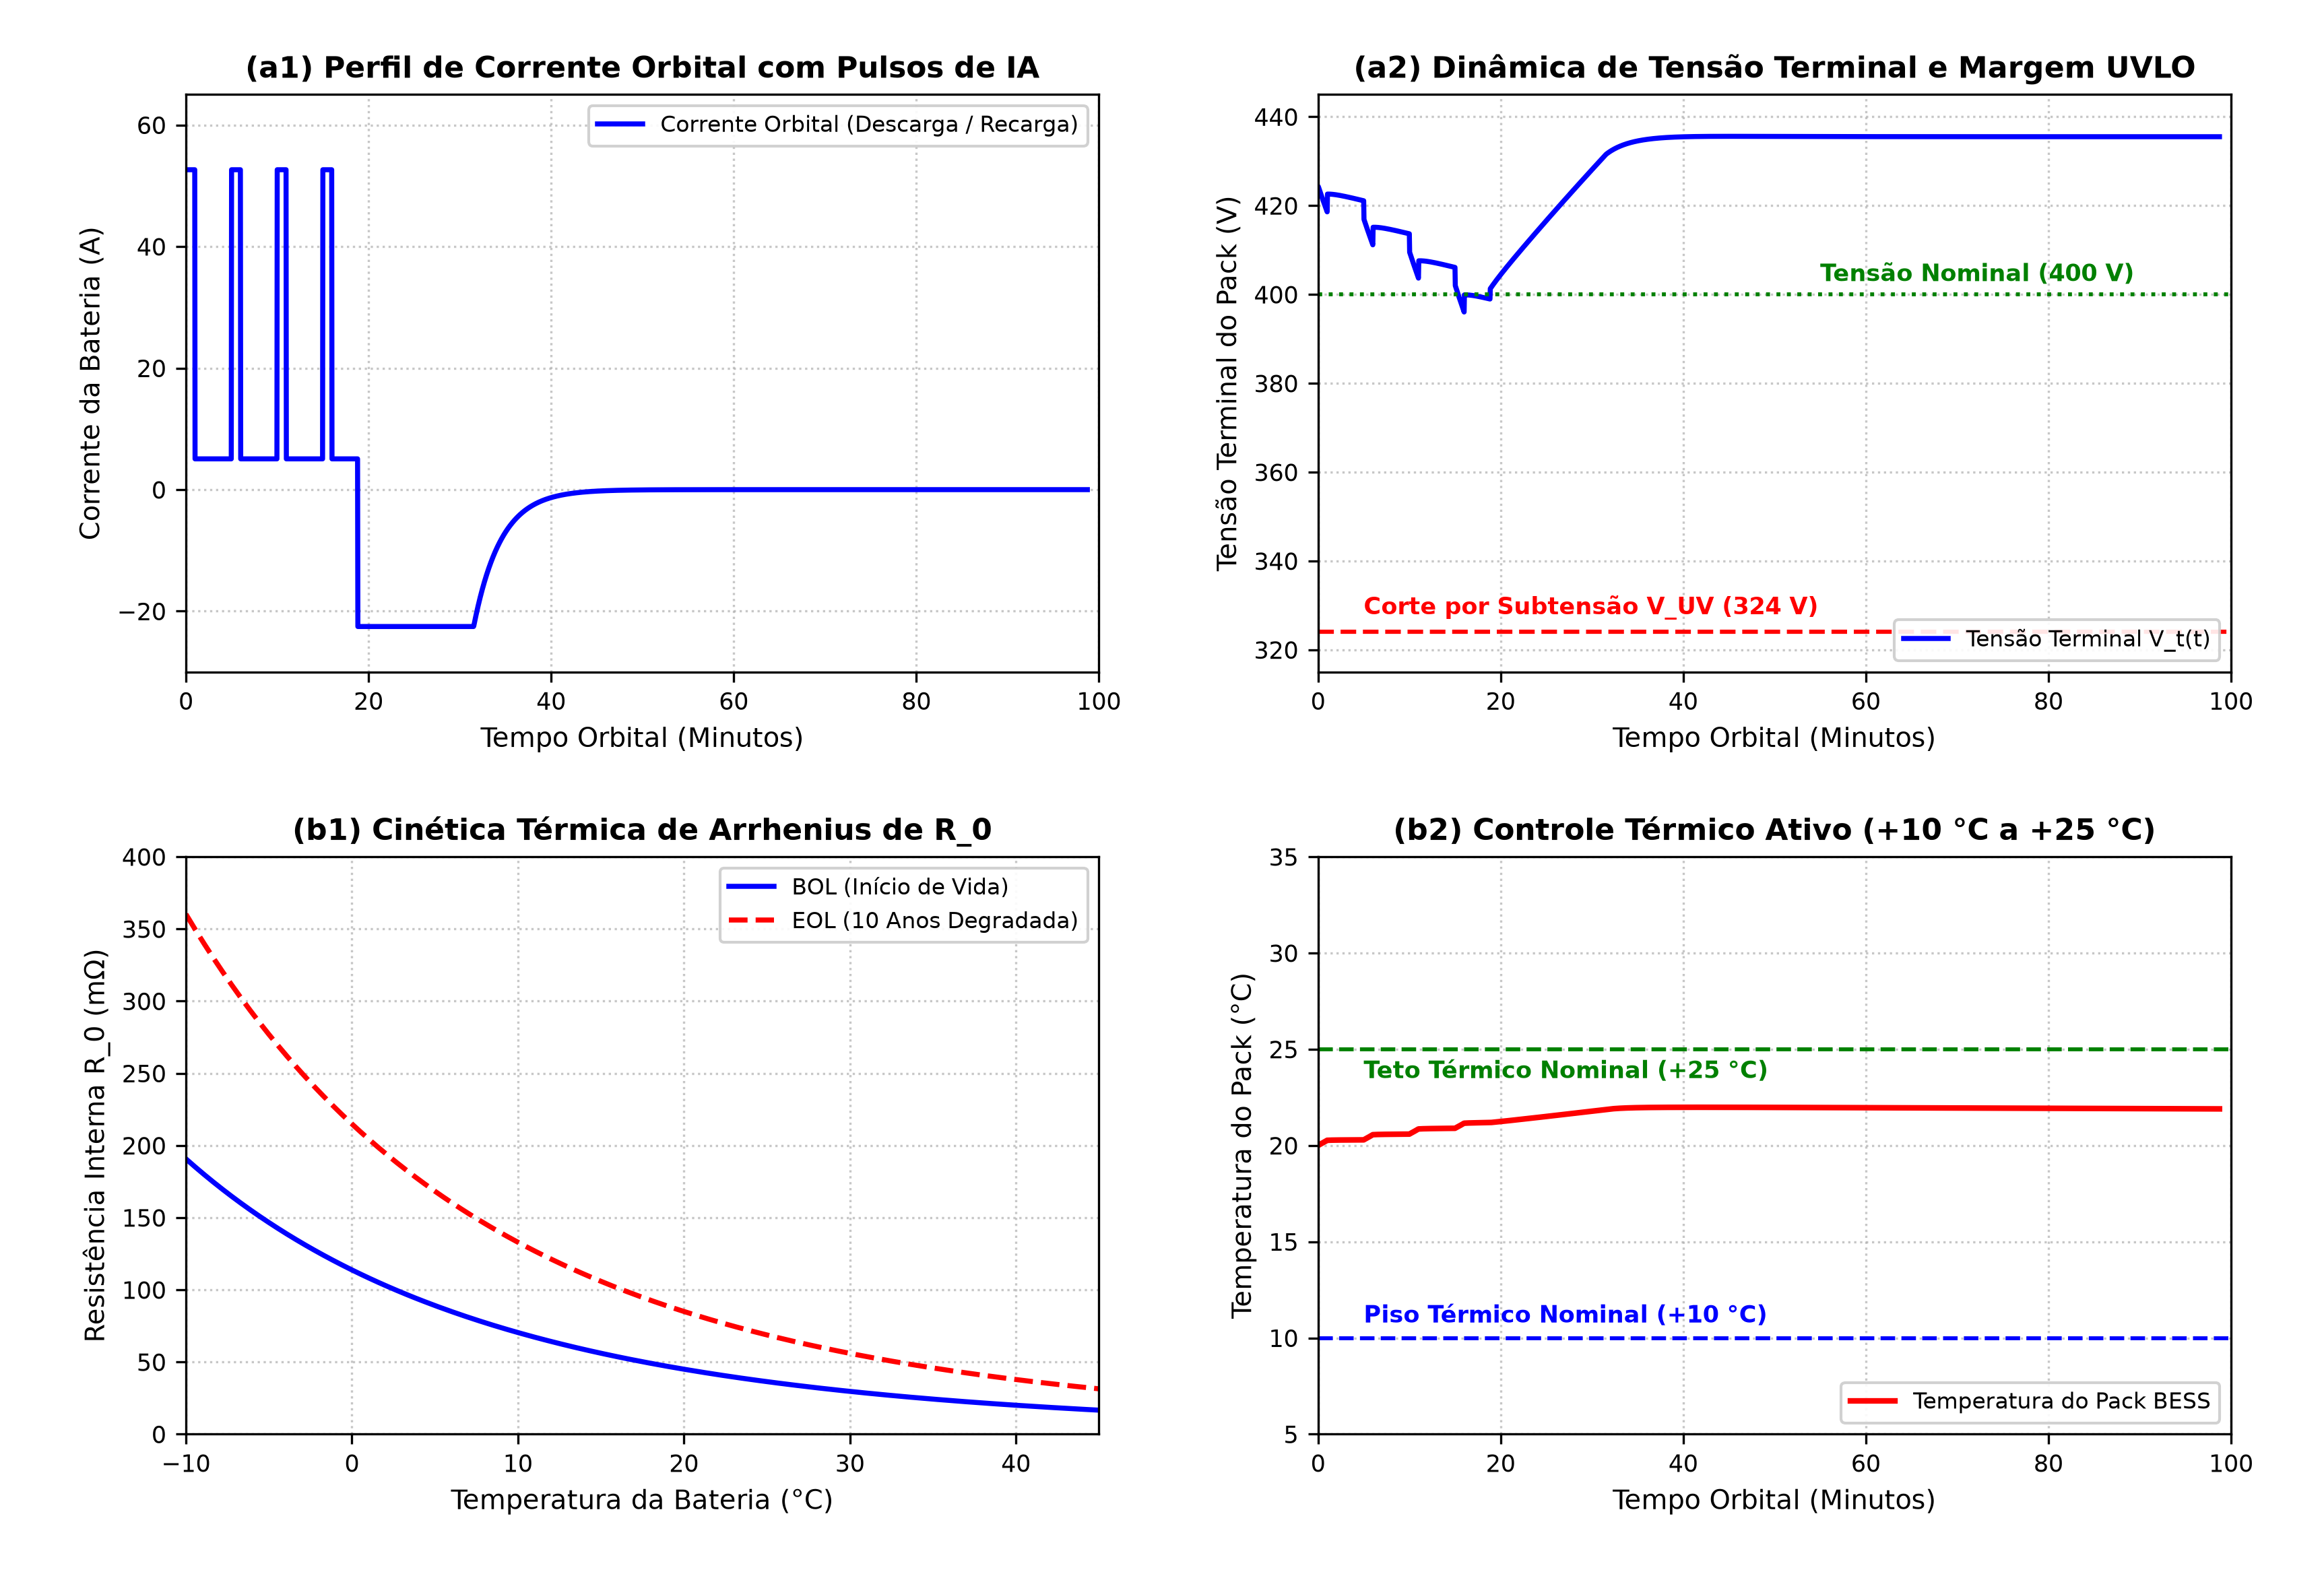
\includegraphics[width=0.82\textwidth]{figuras/figura_3_5_dinamica_dp_eletroquimica.png}
    \caption{Dinâmica eletroquímica e comportamento térmico do BESS de 400~V em órbita LEO (700~km): (a1) perfil de corrente orbital com base de 2~kW e pulsos de IA de 20~kW no eclipse, seguido de recarga solar (-42~A); (a2) resposta da tensão terminal $V_t(t)$ frente a $V_{UV}$; (b1) cinética térmica de Arrhenius de $R_0(T_{bat})$ em BOL e EOL; (b2) temperatura $T_{bat}$ sob controle ativo mantida entre $+10^\circ\text{C}$ e $+25^\circ\text{C}$.}
    \label{fig:dinamica_dp_eletroquimica}
\end{figure}

\subsubsection{Balanço Térmico Consistente: Manta MLI e Aquecedor PWM}

O valor $R_{th,MLI} = 4{,}8\text{ K/W}$ representa o isolamento condutivo-radiativo global entre o invólucro do pack e o chassi [PROVISÓRIO]. O balanço térmico concentrado é dado por:
\begin{equation}
    C_{th,bat} \frac{dT_{bat}(t)}{dt} = P_{loss}(t) + P_{heat}(t) - \frac{T_{bat}(t) - T_{chassis}}{R_{th,MLI}}
    \label{eq:balanco_termico_consistente}
\end{equation}
com $C_{th,bat} = 54.360\text{ J/K}$ ($60\text{ kg}$ NMC, $c_p \approx 906\text{ J/(kg K)}$), $P_{loss} = I_{bat}^2 R_0(T_{bat}) + V_{p1}^2/R_{p1} + V_{p2}^2/R_{p2}$, e aquecedor de sobrevivência modulado em $0 \le P_{heat}(t) \le 300\text{ W}$ ativado termostaticamente entre $+10^\circ\text{C}$ e $+25^\circ\text{C}$.

\subsubsection{Estimação Adaptativa de SoC via AUKF com Adaptação de Sage--Husa}

Para observabilidade sob ruído de sensoriamento ($R_{meas} = 0{,}0225\text{ V}^2$, $150\text{ mV}_{rms}$), formula-se o AUKF com $\mathbf{x}_k = [SoC_k, V_{p1,k}, V_{p2,k}]^T$ ($L = 3$) e $2L+1=7$ pontos sigma (detalhes no Apêndice~C). A adaptação estocástica das covariâncias $\mathbf{Q}_k$ e $\mathbf{R}_k$ segue a recursão de Sage--Husa:
\begin{align}
    \mathbf{R}_k &= (1 - d_k) \mathbf{R}_{k-1} + d_k \left( \nu_k \nu_k^T - \mathbf{P}_{yy,k} \right) \label{eq:sage_husa_r} \\
    \mathbf{Q}_k &= (1 - d_k) \mathbf{Q}_{k-1} + d_k \left[ \mathbf{K}_k \nu_k \nu_k^T \mathbf{K}_k^T + \mathbf{P}_{k|k} - \mathbf{F}_k \mathbf{P}_{k-1|k-1} \mathbf{F}_k^T \right] \label{eq:sage_husa_q}
\end{align}
com sequência de esquecimento $d_k = (1 - b)/(1 - b^{k+1})$ ($b = 0{,}95$) e fatoração triangular de Cholesky. Para garantir a estabilidade numérica incondicional frente a erros de arredondamento de ponto flutuante na OBC de bordo, o algoritmo AUKF implementa duas salvaguardas matriciais fundamentais: (i) simetrização forçada em cada iteração $\mathbf{P} \leftarrow \frac{1}{2}(\mathbf{P} + \mathbf{P}^T)$; e (ii) regularização de Cholesky com clampeamento de covariância (\textit{covariance clamping}), impondo um piso estritamente positivo aos autovalores da matriz de covariância ($\lambda_i \ge \epsilon_{clamp} = 10^{-8}$), prevenindo a divergência numérica ou perda de positividade (\textit{Modo de Falha EST-F05}). A reprodutibilidade matemática das rotinas computacionais é assegurada pela inicialização determinística da semente pseudo-aleatória (\texttt{rng(42)}).

A Figura~\ref{fig:convergencia_aukf_estresse} ilustra a convergência do estimador e o ensaio sob pulso de IA de 50~kW em fim de vida útil (EOL).

\begin{figure}[htbp]
    \centering
    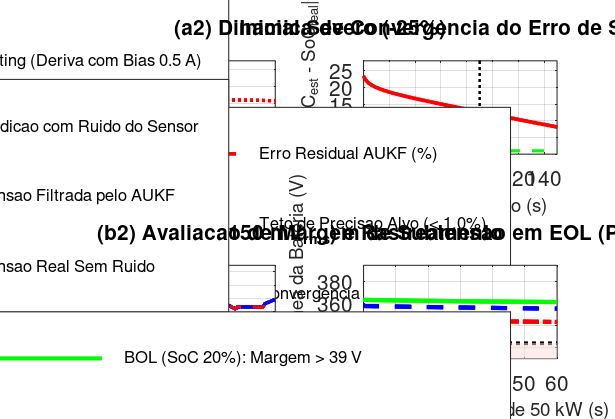
\includegraphics[width=0.82\textwidth]{figuras/figura_3_6_convergencia_aukf_estresse.png}
    \caption{Desempenho do estimador AUKF e resposta de subtensão em EOL: (a1) convergência de SoC com erro inicial de $-25\%$ e comparação com deriva do Coulomb Counting; (a2) erro absoluto $|SoC_{est} - SoC_{real}| < 1{,}0\%$ em $< 90\text{ s}$; (b1) filtragem do ruído de sensoriamento ($150\text{ mV}_{rms}$); (b2) resposta sob pulso de IA de 50~kW (140~A por 60~s) em EOL, contrastando a margem operacional a $SoC = 20\%$ ($> 28\text{ V}$) com o ensaio fora de projeto a $SoC = 2\%$ ($> 10\text{ V}$ antes do corte $V_{UV} = 324\text{ V}$).}
    \label{fig:convergencia_aukf_estresse}
\end{figure}

\subsubsection{Limites de Validação e Modos de Falha do BESS e AUKF}

Os limites operacionais, critérios de erro e os pontos em que o modelo atinge falha catastrófica encontram-se sumarizados na Tabela~\ref{tab:matriz_falhas_bess_aukf}.

\begin{table}[!ht]
\centering
\small
\renewcommand{\arraystretch}{0.85}
\caption{Matriz de Modos de Falha, Limites de Estresse e Mecanismos Críticos do BESS e Estimador AUKF.}
\label{tab:matriz_falhas_bess_aukf}
\resizebox{0.95\textwidth}{!}{%
\begin{tabular}{lp{3.5cm}p{3.5cm}p{3.5cm}p{4.5cm}}
\hline
\textbf{Código} & \textbf{Modo de Falha} & \textbf{Limiar de Entrada em Falha} & \textbf{Efeito Sistêmico Catastrófico} & \textbf{Estratégia de Mitigação Implementada} \\ \hline
\textbf{BAT-F01} & Colapso por Subtensão em EOL & $V_{bat}(t) < 324{,}0\text{ V}$ ($3{,}0\text{ V/cel}$) sob $SoC \le 35\%$ e pulso de 20~kW & Desligamento imediato dos racks de IA por proteção do BMS & \textit{Derating} adaptativo da potência de IA pelo AUKF conforme $R_0(t)$ e $SoC$ \\
\textbf{BAT-F02} & Sobretensão Eletroquímica de Carga & $V_{bat}(t) > 442{,}8\text{ V}$ ($4{,}10\text{ V/cel}$) na saída de eclipse & Degradação do cátodo, gaseificação e risco de inflamação & Transição automática do MPPT para modo de limitação de tensão (CV) \\
\textbf{BAT-F03} & Deposição de Lítio Metálico (\textit{Plating}) & Carga rápida com $T_{bat} < 0^\circ\text{C}$ e corrente $|I_{bat}| > 20\text{ A}$ & Crescimento de dendritos, perfuração do separador e curto interno & Bloqueio compulsório de recarga em subzero e pré-aquecimento com $P_{heat} \le 300\text{ W}$ \\
\textbf{BAT-F04} & Superaquecimento do Pack & $T_{bat} > +45{,}0^\circ\text{C}$ contínua no interior da manta MLI & Decomposição da camada SEI e fuga térmica eletroquímica & Corte do aquecedor PWM e redução do regime de processamento neural \\
\textbf{EST-F05} & Perda de Positividade de Covariância & $\text{det}(\mathbf{P}_{k|k}) \le 0$ ou autovalores negativos em $\mathbf{Q}_k / \mathbf{R}_k$ & Divergência numérica do ganho de Kalman e travamento do OBC & Fatoração de Cholesky, simetrização forçada e piso positivo $\mathbf{P} \leftarrow \text{diag}(\max(\text{diag}(\mathbf{P}), \epsilon))$ \\
\textbf{EST-F06} & Deriva Divergente por Bias de Sensor & Sensor com $\Delta I_{bias} > 0{,}5\text{ A}$ operando por contagem pura & Erro de $SoC > 12\%$ ao final de uma órbita & Correção em malha fechada pelo AUKF baseada na inovação de tensão $\nu_k$ \\ \hline
\end{tabular}%
}
\end{table}

O Quadro~\ref{quadro:parametros_bess_aukf_sintese} sintetiza os parâmetros consolidados de projeto do BESS e do estimador AUKF.

\begin{table}[!ht]
\centering
\small
\renewcommand{\arraystretch}{0.85}
\caption{Parâmetros essenciais de projeto, estresse WCA e classificação epistêmica do BESS e AUKF.}
\label{quadro:parametros_bess_aukf_sintese}
\resizebox{0.95\textwidth}{!}{%
\begin{tabular}{lccccp{5.5cm}}
\hline
\textbf{Parâmetro de Decisão} & \textbf{Símbolo} & \textbf{Mínimo} & \textbf{Nominal} & \textbf{Máximo} & \textbf{Classificação e Justificativa Normativa} \\ \hline
Química Eletroquímica da Célula & Li-ion NMC-811 & 3,00~V (corte) & 3,70~V (nom.) & 4,10~V (teto) & \textbf{[VERIFICÁVEL]} Célula prismática espacial 22,5 Ah; ECSS-E-HB-20-02A \\
Configuração Eletroquímica & $N_s \times N_p$ & 108S1P & 108S1P & 108S1P & \textbf{[CALCULADO]} Arquitetura A (Conexão Direta ao Barramento) \\
Tensão Nominal do Pack & $V_{bat,nom}$ & 324,0~V (3,0 V/cel) & 399,6~V (3,7 V/cel) & 442,8~V (4,1 V/cel) & \textbf{[CALCULADO]} $108 \times 3{,}7\text{ V}$; faixa compatível NASA-HDBK-4007A \\
Capacidade e Energia por Nó & $C_{n,no}, E_{nom,no}$ & 21~Ah / 8,4~kWh & 22,5~Ah / 9,0~kWh & 24~Ah / 9,6~kWh & \textbf{[CALCULADO]} $C_{n} = 9.000\text{ Wh} / 399{,}6\text{ V}$ (Pack de 60 kg) \\
Capacidade e Energia Total (Cluster)& $C_{n,tot}, E_{tot}$ & 420~Ah / 168~kWh & 450,5~Ah / 180~kWh & 480~Ah / 192~kWh & \textbf{[CALCULADO]} Soma dos 20 nós operacionais interligados \\
Energia Utilizável do Nó ($DoD=60\%$)& $E_{util,no}$ & 5,0~kWh & 5,4~kWh & 5,8~kWh & \textbf{[CALCULADO]} $9{,}0\text{ kWh} \times 0{,}60 \times 1{,}0$ ($108\text{ kWh}$ no cluster) \\
Resistência Ôhmica BOL (20°C) & $R_{0,ref}$ & 32,0~m$\Omega$ (a 30°C) & 45,0~m$\Omega$ (a 20°C) & 115,0~m$\Omega$ (a 0°C) & \textbf{[PROVISÓRIO]} Cinética de Arrhenius ($E_a = 0{,}32\text{ eV}$) \\
Resistência Ôhmica EOL (10 anos) & $R_{0,eol}$ & 65,0~m$\Omega$ (a 30°C) & 85,0~m$\Omega$ (a 20°C) & 218,0~m$\Omega$ (a 0°C) & \textbf{[PROVISÓRIO]} Envelhecimento SEI (JUN et al., 2020) \\
Potência Máxima do Aquecedor PWM & $P_{heat,max}$ & 0~W & 150~W & 300~W & \textbf{[CALCULADO]} Teto seguro contra superaquecimento em MLI \\
Resistência Térmica da Manta MLI & $R_{th,MLI}$ & 3,5~K/W & 4,8~K/W & 6,2~K/W & \textbf{[PROVISÓRIO -- NÃO VALIDADO]} Isolamento passivo de vácuo \\
Ruído de Sensoriamento de Tensão & $\sigma_{v,meas}$ & 20~mV$_{rms}$ & 150~mV$_{rms}$ & 300~mV$_{rms}$ & \textbf{[DEPENDENTE DE HARDWARE]} $R_{meas} = (0{,}15\text{ V})^2$ a 400~V \\
Erro Residual Alvo de SoC (AUKF) & $e_{SoC,alvo}$ & -- & -- & 1,20\% & \textbf{[META; NÃO MEDIDA]} Avaliação numérica reprodutível ainda necessária \\ \hline
\end{tabular}%
}
\end{table}

\noindent A integração consistente entre a arquitetura do barramento HVDC de 400~V (Seção~3.1), a geração multijunção de 1~MW sob espectro AM0 (Seção~3.2), o rastreamento MPPT sob gradientes térmicos (Seção~3.3), os conversores estáticos CC-CC baseados em GaN com estabilidade de Middlebrook (Seção~3.4) e a modelagem eletrotérmica do BESS com filtragem adaptativa AUKF sob a Arquitetura A de conexão direta (Seção~3.5) consolida o subsistema elétrico e de armazenamento da espaçonave. Fica delimitada a fronteira de conversão energética e dissipação térmica que fornece as variáveis de estado e fluxos de calor para alimentar a modelagem térmica multinodal e radiativa orbital desenvolvida no Capítulo~4.
